% Options for packages loaded elsewhere
\PassOptionsToPackage{unicode}{hyperref}
\PassOptionsToPackage{hyphens}{url}
%
\documentclass[
]{book}
\usepackage{lmodern}
\usepackage{amssymb,amsmath}
\usepackage{ifxetex,ifluatex}
\ifnum 0\ifxetex 1\fi\ifluatex 1\fi=0 % if pdftex
  \usepackage[T1]{fontenc}
  \usepackage[utf8]{inputenc}
  \usepackage{textcomp} % provide euro and other symbols
\else % if luatex or xetex
  \usepackage{unicode-math}
  \defaultfontfeatures{Scale=MatchLowercase}
  \defaultfontfeatures[\rmfamily]{Ligatures=TeX,Scale=1}
\fi
% Use upquote if available, for straight quotes in verbatim environments
\IfFileExists{upquote.sty}{\usepackage{upquote}}{}
\IfFileExists{microtype.sty}{% use microtype if available
  \usepackage[]{microtype}
  \UseMicrotypeSet[protrusion]{basicmath} % disable protrusion for tt fonts
}{}
\makeatletter
\@ifundefined{KOMAClassName}{% if non-KOMA class
  \IfFileExists{parskip.sty}{%
    \usepackage{parskip}
  }{% else
    \setlength{\parindent}{0pt}
    \setlength{\parskip}{6pt plus 2pt minus 1pt}}
}{% if KOMA class
  \KOMAoptions{parskip=half}}
\makeatother
\usepackage{xcolor}
\IfFileExists{xurl.sty}{\usepackage{xurl}}{} % add URL line breaks if available
\IfFileExists{bookmark.sty}{\usepackage{bookmark}}{\usepackage{hyperref}}
\hypersetup{
  pdftitle={Вступ до R},
  pdfauthor={Юрій Клебан},
  hidelinks,
  pdfcreator={LaTeX via pandoc}}
\urlstyle{same} % disable monospaced font for URLs
\usepackage{color}
\usepackage{fancyvrb}
\newcommand{\VerbBar}{|}
\newcommand{\VERB}{\Verb[commandchars=\\\{\}]}
\DefineVerbatimEnvironment{Highlighting}{Verbatim}{commandchars=\\\{\}}
% Add ',fontsize=\small' for more characters per line
\usepackage{framed}
\definecolor{shadecolor}{RGB}{248,248,248}
\newenvironment{Shaded}{\begin{snugshade}}{\end{snugshade}}
\newcommand{\AlertTok}[1]{\textcolor[rgb]{0.94,0.16,0.16}{#1}}
\newcommand{\AnnotationTok}[1]{\textcolor[rgb]{0.56,0.35,0.01}{\textbf{\textit{#1}}}}
\newcommand{\AttributeTok}[1]{\textcolor[rgb]{0.77,0.63,0.00}{#1}}
\newcommand{\BaseNTok}[1]{\textcolor[rgb]{0.00,0.00,0.81}{#1}}
\newcommand{\BuiltInTok}[1]{#1}
\newcommand{\CharTok}[1]{\textcolor[rgb]{0.31,0.60,0.02}{#1}}
\newcommand{\CommentTok}[1]{\textcolor[rgb]{0.56,0.35,0.01}{\textit{#1}}}
\newcommand{\CommentVarTok}[1]{\textcolor[rgb]{0.56,0.35,0.01}{\textbf{\textit{#1}}}}
\newcommand{\ConstantTok}[1]{\textcolor[rgb]{0.00,0.00,0.00}{#1}}
\newcommand{\ControlFlowTok}[1]{\textcolor[rgb]{0.13,0.29,0.53}{\textbf{#1}}}
\newcommand{\DataTypeTok}[1]{\textcolor[rgb]{0.13,0.29,0.53}{#1}}
\newcommand{\DecValTok}[1]{\textcolor[rgb]{0.00,0.00,0.81}{#1}}
\newcommand{\DocumentationTok}[1]{\textcolor[rgb]{0.56,0.35,0.01}{\textbf{\textit{#1}}}}
\newcommand{\ErrorTok}[1]{\textcolor[rgb]{0.64,0.00,0.00}{\textbf{#1}}}
\newcommand{\ExtensionTok}[1]{#1}
\newcommand{\FloatTok}[1]{\textcolor[rgb]{0.00,0.00,0.81}{#1}}
\newcommand{\FunctionTok}[1]{\textcolor[rgb]{0.00,0.00,0.00}{#1}}
\newcommand{\ImportTok}[1]{#1}
\newcommand{\InformationTok}[1]{\textcolor[rgb]{0.56,0.35,0.01}{\textbf{\textit{#1}}}}
\newcommand{\KeywordTok}[1]{\textcolor[rgb]{0.13,0.29,0.53}{\textbf{#1}}}
\newcommand{\NormalTok}[1]{#1}
\newcommand{\OperatorTok}[1]{\textcolor[rgb]{0.81,0.36,0.00}{\textbf{#1}}}
\newcommand{\OtherTok}[1]{\textcolor[rgb]{0.56,0.35,0.01}{#1}}
\newcommand{\PreprocessorTok}[1]{\textcolor[rgb]{0.56,0.35,0.01}{\textit{#1}}}
\newcommand{\RegionMarkerTok}[1]{#1}
\newcommand{\SpecialCharTok}[1]{\textcolor[rgb]{0.00,0.00,0.00}{#1}}
\newcommand{\SpecialStringTok}[1]{\textcolor[rgb]{0.31,0.60,0.02}{#1}}
\newcommand{\StringTok}[1]{\textcolor[rgb]{0.31,0.60,0.02}{#1}}
\newcommand{\VariableTok}[1]{\textcolor[rgb]{0.00,0.00,0.00}{#1}}
\newcommand{\VerbatimStringTok}[1]{\textcolor[rgb]{0.31,0.60,0.02}{#1}}
\newcommand{\WarningTok}[1]{\textcolor[rgb]{0.56,0.35,0.01}{\textbf{\textit{#1}}}}
\usepackage{longtable,booktabs}
% Correct order of tables after \paragraph or \subparagraph
\usepackage{etoolbox}
\makeatletter
\patchcmd\longtable{\par}{\if@noskipsec\mbox{}\fi\par}{}{}
\makeatother
% Allow footnotes in longtable head/foot
\IfFileExists{footnotehyper.sty}{\usepackage{footnotehyper}}{\usepackage{footnote}}
\makesavenoteenv{longtable}
\usepackage{graphicx}
\makeatletter
\def\maxwidth{\ifdim\Gin@nat@width>\linewidth\linewidth\else\Gin@nat@width\fi}
\def\maxheight{\ifdim\Gin@nat@height>\textheight\textheight\else\Gin@nat@height\fi}
\makeatother
% Scale images if necessary, so that they will not overflow the page
% margins by default, and it is still possible to overwrite the defaults
% using explicit options in \includegraphics[width, height, ...]{}
\setkeys{Gin}{width=\maxwidth,height=\maxheight,keepaspectratio}
% Set default figure placement to htbp
\makeatletter
\def\fps@figure{htbp}
\makeatother
\setlength{\emergencystretch}{3em} % prevent overfull lines
\providecommand{\tightlist}{%
  \setlength{\itemsep}{0pt}\setlength{\parskip}{0pt}}
\setcounter{secnumdepth}{5}
\usepackage{booktabs}
\usepackage{fontspec}
\setmainfont{Arial}
\ifluatex
  \usepackage{selnolig}  % disable illegal ligatures
\fi
\usepackage[]{natbib}
\bibliographystyle{apalike}

\title{Вступ до R}
\author{Юрій Клебан}
\date{2021-04-26}

\begin{document}
\maketitle

{
\setcounter{tocdepth}{1}
\tableofcontents
}
\hypertarget{ux437ux430ux433ux430ux43bux44cux43dux430-ux456ux43dux444ux43eux440ux43cux430ux446ux456ux44f}{%
\chapter*{Загальна інформація}\label{ux437ux430ux433ux430ux43bux44cux43dux430-ux456ux43dux444ux43eux440ux43cux430ux446ux456ux44f}}
\addcontentsline{toc}{chapter}{Загальна інформація}

Увага. Курс у процесі розробки. Матеріали додаватимуться по мірі їх написання та рецензування.


\includegraphics[width=0.75\textwidth,height=\textheight]{images/cover.png}

Курс створено у межах проекту ``Підготовка, обробка та ефективне використання даних для наукових досліджень (на основі R)'', що підтримує Європейський союз за програмою \href{https://houseofeurope.org.ua/}{House of Europe}.

\hypertarget{chapter1}{%
\chapter{Вступ до курсу}\label{chapter1}}

\hypertarget{ux43fux43bux430ux43d}{%
\section*{План}\label{ux43fux43bux430ux43d}}
\addcontentsline{toc}{section}{План}

\begin{itemize}
\tightlist
\item
  \protect\hyperlink{chapter11}{Що таке R?}
\item
  \protect\hyperlink{chapter12}{Історія створення R}
\item
  \protect\hyperlink{chapter13}{Основи роботи з R}

  \begin{itemize}
  \tightlist
  \item
    \protect\hyperlink{chapter131}{R Project}

    \begin{itemize}
    \tightlist
    \item
      \protect\hyperlink{chapter1311}{Завантаження та інсталяція R}
    \item
      \protect\hyperlink{chapter1312}{Перший запуск R GUI}
    \item
      \protect\hyperlink{chapter1313}{Поняття робочого простору}
    \item
      \protect\hyperlink{chapter1314}{Поняття робочого каталогу}
    \item
      \protect\hyperlink{chapter1315}{Допомога (help/?)}
    \end{itemize}
  \item
    \protect\hyperlink{chapter132}{Робота з R Studio}

    \begin{itemize}
    \tightlist
    \item
      \protect\hyperlink{chapter1321}{Завантаження та інсталяція RStudio Desktop}
    \item
      \protect\hyperlink{chapter1322}{Створення першого проекту в RStudio}
    \end{itemize}
  \item
    \protect\hyperlink{chapter133}{Робота з Jupyter Notebook}
  \item
    \protect\hyperlink{chapter134}{Огляд додаткових IDE та сервісів для роботи з R}
  \end{itemize}
\item
  \protect\hyperlink{chapter14}{Основи роботи з пакетами в R}

  \begin{itemize}
  \tightlist
  \item
    \protect\hyperlink{chapter141}{Команди для роботи з пакетами}
  \item
    \protect\hyperlink{chapter142}{Робота з пакетами в RStudio}
  \end{itemize}
\end{itemize}

\begin{center}\rule{0.5\linewidth}{0.5pt}\end{center}

\hypertarget{chapter11}{%
\section{Що таке R?}\label{chapter11}}

R є поширеною мовою програмування для роботи з даними (\texttt{DataScience}) та машинного навчання (\texttt{Machine\ Learning}). Але Ви можете скористатися засобами R і для простіших задач: обчислення, візуалізація даних.

Синтаксис мови програмування R є досить простим для вивчення та використання, а широкий набір готових пакетів дозволяє використати готові розробки для виіршення широкого спектру задач від статистичних обчислень до навчання нейронних мереж для розпізнавання/класифікації зображень.

Важливо відмітити, що мова програмування R є безкоштовною (\texttt{free}) і має відкритий код (\texttt{open\ source}).

R має ряд корисних властивостей, серед яких варто виділити:

\begin{itemize}
\item
  \textbf{Візуалізація даних}. Побудова різноманітих видів графіків, робота з мапами, широкий спектр бібліотек та налаштувань до них.
\item
  \textbf{Повторне використання коду}. На відміну від електронних таблиць, що мають обмеження на кількість спостережень (наприклад, MS Excel), R дозволяє працювати з великими масивами даних та перезапускати обчислення у потрібний момент не створюючи додаткових копій даних.
\item
  \textbf{Машинне навчання}. R дозволяє використати для побудови, навчання та тестування моделей, а також оптимізації гіперпараметрів та відбору факторів дуже велику кількість алгоритмів. Існують також спеціальні пакети, що об'єднують у собі усі описані функції та алгоритми, наприклад, \texttt{caret} та \texttt{mlr}.
\item
  \textbf{Автоматизація}. Написаний код та проекти можна перетворити у готові до публікації та впровадження продукти (deployment) або використовувати напрацьовані алгоритми для швидкого вирішення схожих задач (pipeline).
\end{itemize}

Також можна виділити досить корисні фічі \textbf{Розробка веб-застосунків} та \textbf{Звітність}, адже, використовуючи спеціальні бібліотеки (\texttt{shiny}, \texttt{shinydashboard}, \texttt{flexdashboard}, \texttt{rmarkdown}, \texttt{knitr} тощо), результати виконаної роботи можна ``оживити'' або сформувати ``на льоту'' готові до презентації документи.

\begin{center}\rule{0.5\linewidth}{0.5pt}\end{center}

\hypertarget{chapter12}{%
\section{Історія створення R}\label{chapter12}}

Мова програмування \texttt{R} виникла як продовження статистичної мови \texttt{S}. Назва мови \texttt{S} була обрана аналогічно до \texttt{C}. Створена \texttt{S} була у 1976 році компанією \texttt{Bell\ Labs}. Мова \texttt{S} мала кілька версій і широко використовувалася для комерційного програмування. Найпотужнішою була версія \texttt{S-Plus}, що мала реалізацію за досить немалу кількість функцій під \texttt{Windows} та \texttt{Unix}-платформи, що стримувало її розвиток. Саме в цей момент розпочинається історія \texttt{R}.

Влітку 1993 року двоє молодих новозеландських вчених анонсували свлю нову розробку, яку вони назвали \texttt{R} (є інформація, що буква ``R'' була обрана тому, що вона стоїть перед ``S'' у латинському алфавіті, тут є аналогія з мовою ``C'', якій передувала мова ``B'') \citep{R-stats-book}. За задумом авторів (Robert Gentelman та Ross Ihaka) це повинна була бути нова реалізація мови \texttt{S}, що відрізнялася від \texttt{S-Plus} деякими деталями, наприклад, роботою з локальними та глобальними змінними, пам'яттю тощо. Фактично було створено нову мову, що відгалуджується від \texttt{S}.

Проект з самого початку розвивався досить повільно, але коли у команди розробників \texttt{R} з'явлися ресурси, в тому числі зручна системи створення розширень (пакетів), все більше аналітиків, статистиків, вчених, програмістів почало переходити з \texttt{S-Plus} на \texttt{R}. Коли були усунуті проблеми роботи з пам'яттю перших версій \texttt{R}, на цю мову почали переходити користувачі інших статистичних пакетів (SAS, Stata, SYSSTAT).

Кількість книг та публікацій у мережі Інтернет по роботі з R постійно зростає разом із зацікавленням молодих і вже досвідчених спеціалістів зі сфери ІТ темою науки про дані, машинним навчанням, аналітикою для бізнесу, охорони здоров'я тощо.

\begin{center}\rule{0.5\linewidth}{0.5pt}\end{center}

\hypertarget{chapter13}{%
\section{Основи роботи з R}\label{chapter13}}

\hypertarget{chapter131}{%
\subsection{R Project}\label{chapter131}}

\texttt{R} є безкоштовним програмним забезпеченням, що розповсюджується за умовами \href{https://www.r-project.org/COPYING}{GNU General Public License}. Код, написаний на \texttt{R} компілюється та запускається на різних платформах: UNIX, Windows, MacOS \citep{R-base}.

\hypertarget{chapter1311}{%
\subsubsection{Завантаження та інсталяція R}\label{chapter1311}}

Для завантаження актуальної версії R варто перейти на сайт проекту \url{https://cran.r-project.org/}.

На сайті обираємо завантаження \texttt{R} для потрібної операційної системи. У межах курсу ми вокристовуємо \texttt{ОС\ Windows}, проте на синтаксис мови програмування та процес написання коду це не впливає:

\begin{figure}

\includegraphics[width=10.15in]{images/chapter1/r_gui_1} \caption{Завантаження R. Вибір ОС}\label{fig:unnamed-chunk-1}
\end{figure}

У наступному вікні клікаємо на \textbf{install R for the first time}:

\begin{figure}

\includegraphics[width=10.32in]{images/chapter1/r_gui_2} \caption{Завантаження R. Перша інсталяція}\label{fig:unnamed-chunk-2}
\end{figure}

Далі обираємо \textbf{Download R 4.X.X for Windows}, де \texttt{4.X.X} версія \texttt{R}, яка може бути відмінною на момент вивчення курсу:

\begin{figure}

\includegraphics[width=10.92in]{images/chapter1/r_gui_3} \caption{Завантаження R. Завантаження версії для ОС}\label{fig:unnamed-chunk-3}
\end{figure}

Після завантаження файлу інсталяції потрібно його запустити. Зазвичай завантажений файл можна побачити у лівому нижному кутку браузера або у розділі ``Завантаження'' Вашого браузера. Наприклад, у браузері \texttt{Google\ Chrome} знайти цей пункт меню так:

\begin{figure}

\includegraphics[width=4.56in]{images/chapter1/chrome_download_button} \caption{Завантаження R. Розділ "Завантаження" у Google Chrome}\label{fig:unnamed-chunk-4}
\end{figure}

Процес інсталяції ПЗ не відрізняється від інших програм і детального опису не потребує. Основним тут є запам'ятати шлях встановлення проекту або ``відмітити галочками'' пункти щодо публікації на \emph{Робочий стіл} чи у меню швидкого доступу ярликів для того, щоб знайти файли запуску.

\hypertarget{chapter1312}{%
\subsubsection{Перший запуск R GUI}\label{chapter1312}}

За замовчуванням під час інсталяції пропонується шлях \texttt{C:\textbackslash{}Program\ Files\textbackslash{}R\textbackslash{}R-4.X.X}.

Для запуску \texttt{R\ GUI} (стандартного графічного інтерфейсу для роботи з \texttt{R}) потрібно зайти у папку \texttt{bin\textbackslash{}x64} (або \texttt{i386}, якщо у Вас 32-х розрядна ОС) та запустити файл \texttt{Rgui.exe}.

Вигляд вікна \texttt{R\ GUI} зображено нижче:

\begin{figure}
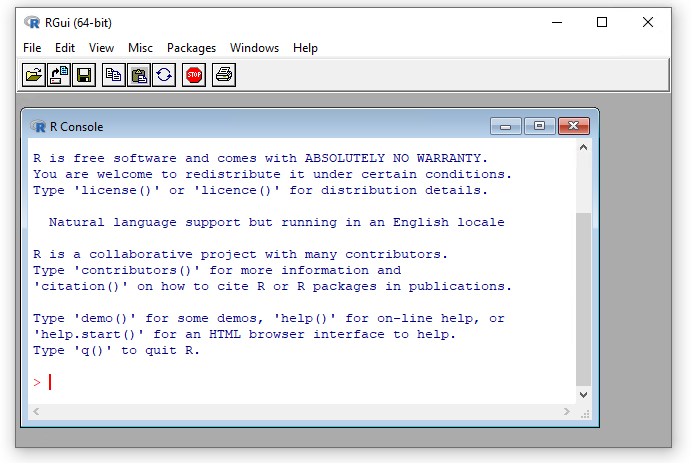
\includegraphics[width=9.61in]{images/chapter1/r_gui_4} \caption{Вигляд головного вікна RGui}\label{fig:unnamed-chunk-5}
\end{figure}

\emph{GUI} (\emph{G}raphical \emph{U}ser \emph{I}nterface) - набір візуальних компонентів для інтерактивної взаємодії користувача з програмним забезпеченням.

У вікні \texttt{R\ Console} можна вводити команди/інструкції \texttt{R}, що будуть виконуватися:

Результати виконання команд зберігаються у памяті програми і можуть бути використані у наступних блоках коду:

\begin{figure}
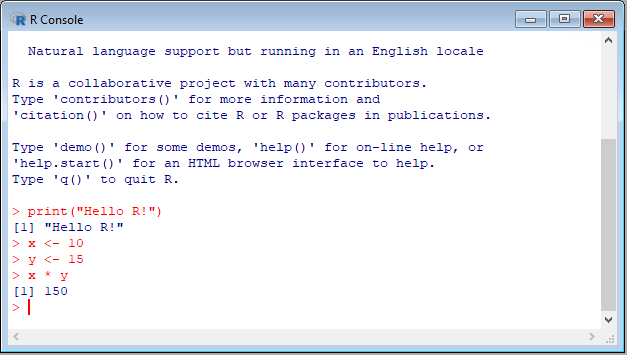
\includegraphics[width=8.71in]{images/chapter1/r_gui_5} \caption{Вигляд консолі для команд RGui}\label{fig:unnamed-chunk-6}
\end{figure}

Середовище \texttt{R\ GUI} має широкий спектр функцій і дозволяє написати будь-якого рівня складності проекти на R, проте він є лише базовою графічною обгорткою для \texttt{R}. Розглянемо інші зручніші середовища для написання \texttt{R}-коду.

\hypertarget{chapter1313}{%
\subsubsection{Поняття робочого простору}\label{chapter1313}}

У процесі виконання коду створені об'єкти/змінні та функції зберігаються у поточній сесії. У \texttt{R} є можливість переглянути список збережних елментів, видалити усі або окремі, зберегти стан поточної сесії диск та завантажити його пізніше, щоб не проходти усі етапи виконання коду повторно \emph{(інколи дуже складний код може виконувати досить довго і збереження проміжних результатів може бути хорошим рішенням)}.

Для прикладу створимо дві змінні \texttt{var1}, \texttt{var2} та виведемо на консоль їх значення:

\begin{Shaded}
\begin{Highlighting}[]
\NormalTok{var1 }\OtherTok{\textless{}{-}} \DecValTok{10}
\NormalTok{var2 }\OtherTok{\textless{}{-}} \FunctionTok{sqrt}\NormalTok{(}\DecValTok{15}\NormalTok{)}
\NormalTok{var1}
\end{Highlighting}
\end{Shaded}

\begin{verbatim}
## [1] 10
\end{verbatim}

\begin{Shaded}
\begin{Highlighting}[]
\NormalTok{var2}
\end{Highlighting}
\end{Shaded}

\begin{verbatim}
## [1] 3.872983
\end{verbatim}

Для того аби переглянути список змінних у поточній сесії варто скористатися \textbf{\texttt{ls()}}:

\begin{Shaded}
\begin{Highlighting}[]
\FunctionTok{ls}\NormalTok{()}
\end{Highlighting}
\end{Shaded}

\begin{verbatim}
## [1] "var1" "var2"
\end{verbatim}

Якщо виникає потреба очистити робочий простір і звільними пам'ять використовується команда \texttt{rm()}. Так, щоб очистити усі змінні можна скористатися \texttt{rm(list\ =\ ls())}, якщо ж Ви хочете видалити якусь одну/дві змінних, то просто вкажіть імена:

\begin{Shaded}
\begin{Highlighting}[]
\FunctionTok{rm}\NormalTok{(}\AttributeTok{list =} \FunctionTok{c}\NormalTok{(}\StringTok{"var1"}\NormalTok{))}
\FunctionTok{ls}\NormalTok{()}
\end{Highlighting}
\end{Shaded}

\begin{verbatim}
## [1] "var2"
\end{verbatim}

Таким чином, після виконання коду вище, залишиться лише змінна \texttt{var2}.

Зберігання образу (\texttt{image}) робочого простору на диск здыйснюэться за допомогою команди \texttt{save.image("шлях\ до\ файлу.RData")}, а його зчитування за допомогою \texttt{load("шлях\ до\ файлу.RData")}:

\begin{Shaded}
\begin{Highlighting}[]
\CommentTok{\# Clear workspace}
\FunctionTok{rm}\NormalTok{(}\AttributeTok{list =} \FunctionTok{ls}\NormalTok{())}

\CommentTok{\# declare data}
\NormalTok{a }\OtherTok{\textless{}{-}} \DecValTok{10}
\NormalTok{b }\OtherTok{\textless{}{-}}\NormalTok{ a }\SpecialCharTok{+} \DecValTok{15}

\CommentTok{\# Save image to file}
\FunctionTok{save.image}\NormalTok{(}\StringTok{"tmp.RData"}\NormalTok{)}
\end{Highlighting}
\end{Shaded}

\begin{Shaded}
\begin{Highlighting}[]
\CommentTok{\# Clear workspace}
\FunctionTok{rm}\NormalTok{(}\AttributeTok{list =} \FunctionTok{ls}\NormalTok{())}

\CommentTok{\# load image to file}
\FunctionTok{load}\NormalTok{(}\StringTok{"tmp.RData"}\NormalTok{)}

\FunctionTok{print}\NormalTok{(a)}
\end{Highlighting}
\end{Shaded}

\begin{verbatim}
## [1] 10
\end{verbatim}

\begin{Shaded}
\begin{Highlighting}[]
\FunctionTok{print}\NormalTok{(b)}
\end{Highlighting}
\end{Shaded}

\begin{verbatim}
## [1] 25
\end{verbatim}

У прикладі 2 не створюєть жодного параметра, проте вони збережні у файлі сесії.

Для того аби зберегти та зчитати окремий об'єкт, а не всі елементи сесії у \texttt{R} э спеціальний формат \texttt{.RDS}, який реалізовується методами \texttt{saveRDS(об\textquotesingle{}єкт,\ file="шлях\_файлу.rds")} та \texttt{readRDS(file="шлях\_файлу.rds")}.

\hypertarget{chapter1314}{%
\subsubsection{Поняття робочого каталогу}\label{chapter1314}}

Робота в будь-якому середовищі передбачає зв'язок із поточним каталогом, відносно якого будуються шляхи до файлів. Звичайно можна писати завжди повний шлях до файла, проте такий підхід є досить негнучким і під час перенесення коду між ПК створює чимало проблем розробникам.

Для визначення базового каталогу \texttt{R} в поточній сесії використовують команду \texttt{getwd()}. Якщо Ви користуєтеся \texttt{RStudio} та створили проект, то цей каталог буде відповідати повному шляху до папки проекту:

\begin{Shaded}
\begin{Highlighting}[]
\FunctionTok{getwd}\NormalTok{()}
\end{Highlighting}
\end{Shaded}

\begin{verbatim}
## [1] "E:/Repos/YuRa/r-intro"
\end{verbatim}

Для того аби змінити поточний робочий каталог використовують команду \texttt{setwd(шлях)}. Після запуску цієї команди функцій \texttt{getwd()} буде вказутивати уже на нову адресу/шлях.

Варто знати та вміти будувати \textbf{абсолютні} та \textbf{відносні} шляхи до каталогів та файлів, ці знання корисні для роботи з усіма мовами програмування та більшістю ПЗ для роботи з даними.

Для запису шляху у ОС Windows можна скористатися 2-ма способами:

\begin{itemize}
\tightlist
\item
  \texttt{/} - \textbf{\emph{слеш}}, записується як один знак;
\item
  \texttt{\textbackslash{}\textbackslash{}} - \textbf{\emph{бекслеш}}, записується як два знаки.
\end{itemize}

У прикладі нижче обидва шляхи ведуть до тієї ж папки (\texttt{drive} - буква диска):

\begin{Shaded}
\begin{Highlighting}[]
\FunctionTok{setwd}\NormalTok{(}\StringTok{"drive:/folder1/folder2/"}\NormalTok{)}
\FunctionTok{setwd}\NormalTok{(}\StringTok{"drive:}\SpecialCharTok{\textbackslash{}\textbackslash{}}\StringTok{folder1}\SpecialCharTok{\textbackslash{}\textbackslash{}}\StringTok{folder2}\SpecialCharTok{\textbackslash{}\textbackslash{}}\StringTok{"}\NormalTok{)}
\end{Highlighting}
\end{Shaded}

Для перегляду інформації про наявні каталоги та файли у поточній робочій папці можна скористатися командою \texttt{dir()} або \texttt{list.files()}:

\begin{Shaded}
\begin{Highlighting}[]
\FunctionTok{dir}\NormalTok{()}
\end{Highlighting}
\end{Shaded}

\begin{verbatim}
##  [1] "_bookdown.yml"       "_bookdown_files"     "_output.yml"        
##  [4] "01-chapter1.Rmd"     "01-chapter1_files"   "01-intro_files"     
##  [7] "02-chapter2.Rmd"     "02-chapter2_files"   "03-chapter3.Rmd"    
## [10] "06-chapter6.Rmd"     "07-references.Rmd"   "book.bib"           
## [13] "css"                 "favicon.ico"         "images"             
## [16] "inc"                 "index.md"            "index.Rmd"          
## [19] "index.utf8.md"       "packages.bib"        "preamble.tex"       
## [22] "r-intro.log"         "r-intro.rds"         "README.md"          
## [25] "render_commands"     "renderf147d616f.rds" "RIntro.Rproj"       
## [28] "tmp.RData"
\end{verbatim}

\begin{Shaded}
\begin{Highlighting}[]
\FunctionTok{list.files}\NormalTok{()}
\end{Highlighting}
\end{Shaded}

\begin{verbatim}
##  [1] "_bookdown.yml"       "_bookdown_files"     "_output.yml"        
##  [4] "01-chapter1.Rmd"     "01-chapter1_files"   "01-intro_files"     
##  [7] "02-chapter2.Rmd"     "02-chapter2_files"   "03-chapter3.Rmd"    
## [10] "06-chapter6.Rmd"     "07-references.Rmd"   "book.bib"           
## [13] "css"                 "favicon.ico"         "images"             
## [16] "inc"                 "index.md"            "index.Rmd"          
## [19] "index.utf8.md"       "packages.bib"        "preamble.tex"       
## [22] "r-intro.log"         "r-intro.rds"         "README.md"          
## [25] "render_commands"     "renderf147d616f.rds" "RIntro.Rproj"       
## [28] "tmp.RData"
\end{verbatim}

\hypertarget{chapter1315}{%
\subsubsection{Допомога (help/?)}\label{chapter1315}}

Для отримання швидкої довідки в \texttt{R} варто скористатися функціє \texttt{help(назва\_об\textquotesingle{}єкта\_або\_функції)} або \texttt{?назва\_об\textquotesingle{}єкта\_або\_функції}:

\begin{Shaded}
\begin{Highlighting}[]
\CommentTok{\# Get help for intersect() function}
\FunctionTok{help}\NormalTok{(intersect)}
\end{Highlighting}
\end{Shaded}

Якщо є потреба отримати інформацію про пакет скористайтеся:

\begin{Shaded}
\begin{Highlighting}[]
\FunctionTok{help}\NormalTok{(}\AttributeTok{package =} \StringTok{"stats"}\NormalTok{)}
\end{Highlighting}
\end{Shaded}

\hypertarget{chapter132}{%
\subsection{Робота з R Studio}\label{chapter132}}

\hypertarget{chapter1321}{%
\subsubsection{Завантаження та інсталяція RStudio Desktop}\label{chapter1321}}

\textbf{RStudio} - це інтегроване середовище розробки для \texttt{R}. Воно включає у себе консоль, підсвічування синтаксису (підказки), прямий запуск коду, інструменти для візуалізації графіків, html-коду, історію виконаних команд, відлагоджування коду, управління робочими просторами, підтримка різних видів розмітки та багато іншого. RStudio має версію з відкритим кодом та комерційну версію для \texttt{Windows}, \texttt{Linux} та \texttt{Mac}, а також веб-версію для серверів на Linux \texttt{RStudio\ Server} та \texttt{RStudio\ Server\ Pro} \citep{R-studio-site}.

IDE (\texttt{integrated\ development\ environment}) - комплексне програмне рішення для розробки програмного забезпечення. Зазвичай, складається з редактора початкового коду, інструментів для автоматизації складання та відлагодження програм. Більшість сучасних середовищ розробки мають можливість автодоповнення коду. Wikipedia

Завантажити продукти можна з сайту \url{https://rstudio.com}. Щоб знайти середовище, яке ми будемо використовувати під час вивчення курсу варто виконати наступні кроки:

\begin{enumerate}
\def\labelenumi{\arabic{enumi}.}
\tightlist
\item
  У головному меню сайту обрати \texttt{Products\ \textgreater{}\ RStudio}.
\item
  Знаходимо на сторінці кнопку для завантаження програми \texttt{RStudio\ Desktop} версії \texttt{Open\ Source} та натискаємо \textbf{DOWNLOAD RSTUDIO DESKTOP}:
\end{enumerate}

\begin{figure}
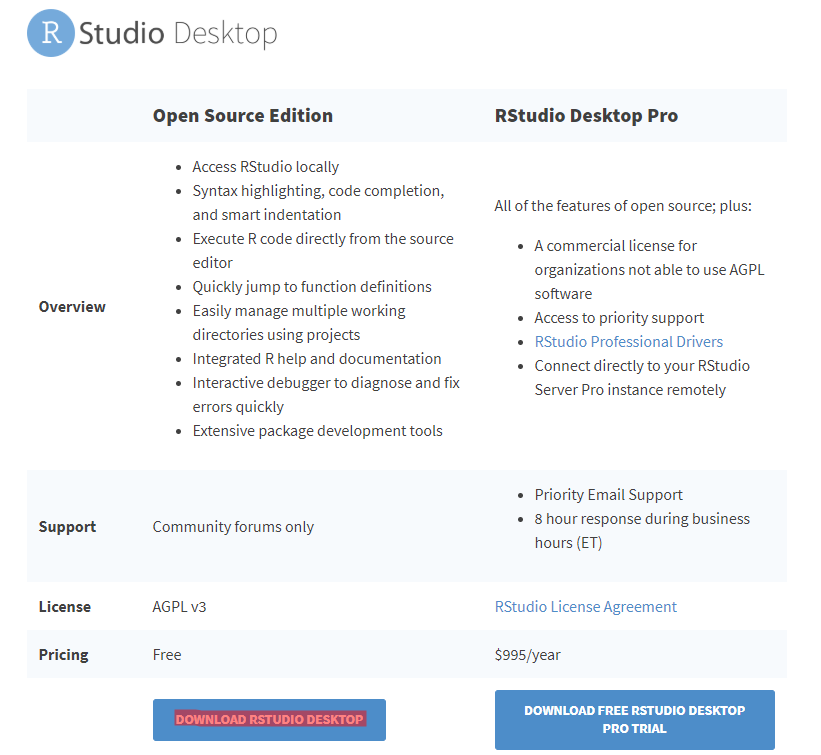
\includegraphics[width=11.4in]{images/chapter1/rstudio_1} \caption{Вибір версії RStudio Desktop}\label{fig:unnamed-chunk-13}
\end{figure}

\begin{enumerate}
\def\labelenumi{\arabic{enumi}.}
\setcounter{enumi}{2}
\tightlist
\item
  Далі обираємо завантаження безкоштовної версії \texttt{RStudio\ Desktop} з наданого переліку:
\end{enumerate}

\begin{figure}
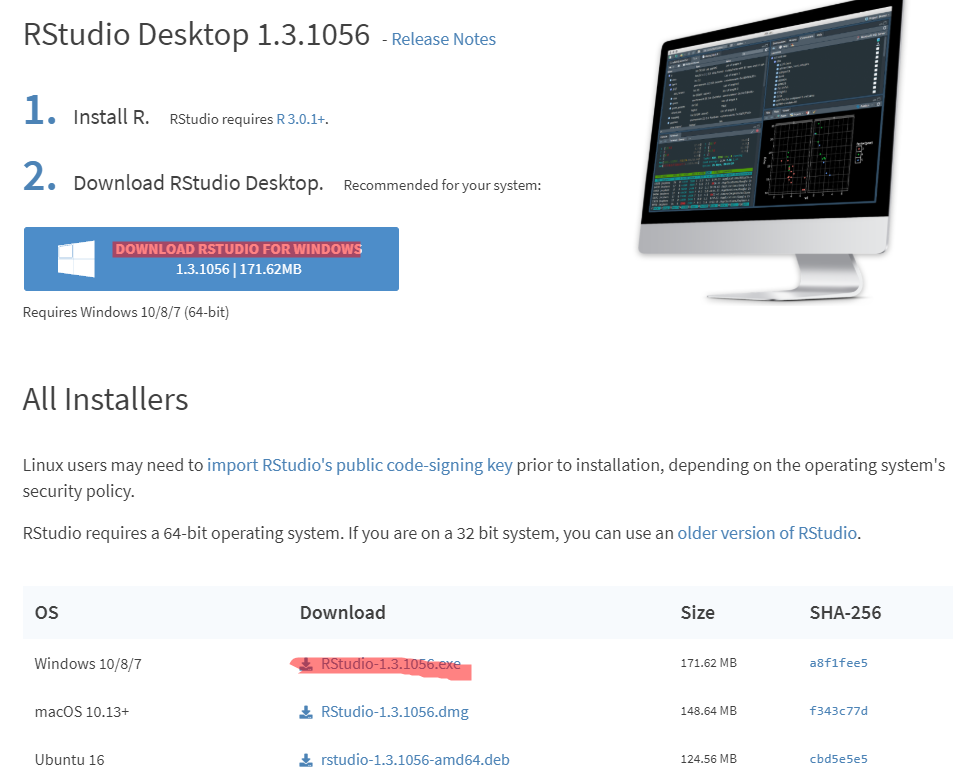
\includegraphics[width=13.38in]{images/chapter1/rstudio_2} \caption{Завантаження RStudio Desktop}\label{fig:unnamed-chunk-14}
\end{figure}

Після завантаження запускаємо інсталятор \texttt{RStudio}. Особливих кроків у цьому процесі немає.

Після запуску IDE RStudio зазвичай складається з 3-х або 4-х блоків:
* Файл, з яким працювали останнім (зліва зверху).
* Консоль для введення коду та виведення результатів (зліва знизу).
* Змінні середовища (\texttt{Environment}) (справа зверху) + Історія команд (\texttt{History}), Зєднання з зовнішніми ресурсами даних, наприклад, бази даних (\texttt{Connections}), навчальна інструкція (\texttt{Tutorial}).
* Файли каталогу або проекту (\texttt{Files}), Інстальовані пакети (\texttt{Packages}), Допомога (\texttt{Help}), Візуалізація результатів (\texttt{Plots}, \texttt{Viewer}).

\begin{figure}
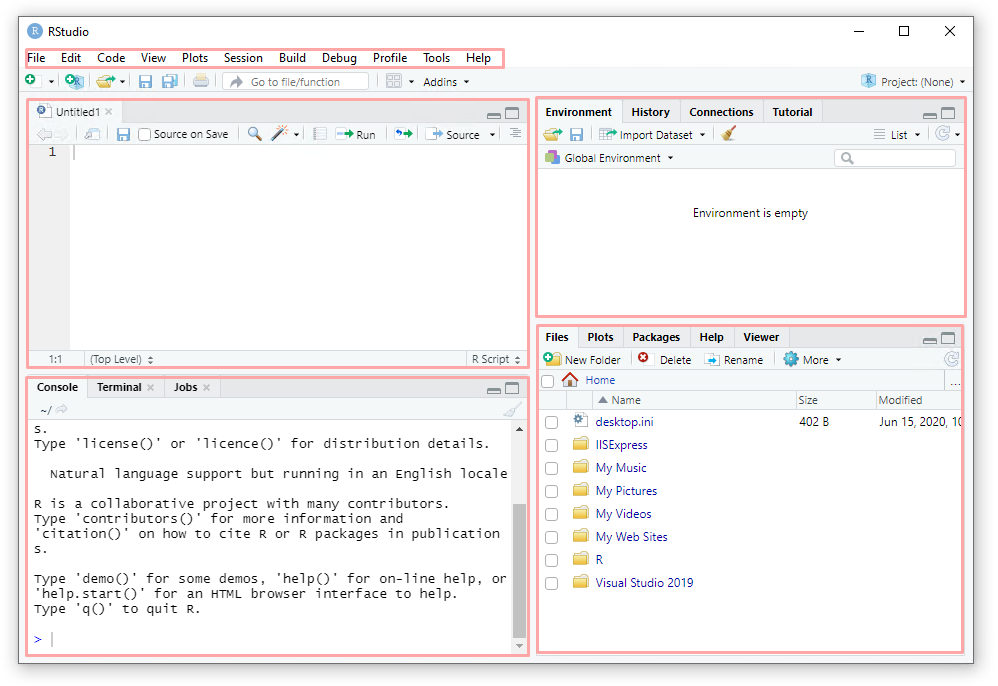
\includegraphics[width=13.86in]{images/chapter1/rstudio_3} \caption{Головне вікно RStudio Desktop}\label{fig:unnamed-chunk-15}
\end{figure}

Для першої демонстрації роботи виконаємо у консолі 2 рядки коду:

\begin{figure}
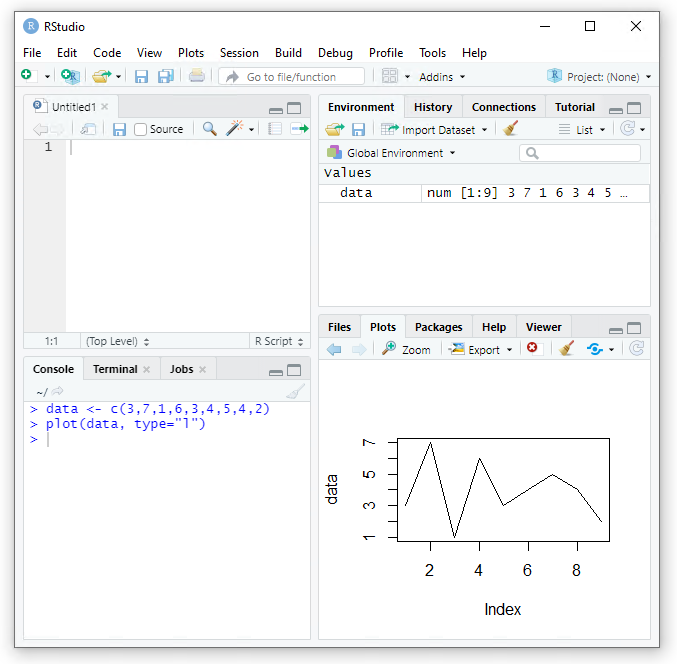
\includegraphics[width=9.4in]{images/chapter1/rstudio_4} \caption{Приклад написання коду в RStudio Desktop}\label{fig:unnamed-chunk-16}
\end{figure}

Перший рядок з кодом \texttt{data\ \textless{}-\ c(3,7,1,6,3,4,5,4,2)} створює у пам'яті колекцію чисел. Зверніть увагу, що у блоці \textbf{Environments} відобраюаться усі змінні, що уснують у поточному робочому просторі (про це буде далі).

Другий рядок \texttt{plot(data,\ type="l")} дозволяє побудувати простий лінійний графік (\texttt{type="l"\ -\ linear,\ "p"\ -\ point}, \texttt{help(plot)} для деталей). Графіки, що ``промальовуються'' як картинки выдображаються у блоці \textbf{Plots}. Якщо ж графік має більш складну візуалізацію з інтерактивними елементами, що використовують уже засоби html/css/js, то він буде відображений у блоці \textbf{View}.

Якщо перемкнутися на вкладку \textbf{History}, то ми побачимо перелік раніше виконаних команд.

Для швидкого ``гортання'' уже виконаних раніше команд на консолі (\emph{Console}) можна скористатися клавішами Up/Down на клавіатурі:
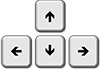
\includegraphics{images/chapter1/arrow_keys.png}

\hypertarget{ux441ux442ux432ux43eux440ux435ux43dux43dux44f-ux43fux435ux440ux448ux43eux433ux43e-ux43fux440ux43eux435ux43aux442ux443-ux432-rstudio-chapter1322}{%
\subsubsection{Створення першого проекту в RStudio \{chapter1322\}}\label{ux441ux442ux432ux43eux440ux435ux43dux43dux44f-ux43fux435ux440ux448ux43eux433ux43e-ux43fux440ux43eux435ux43aux442ux443-ux432-rstudio-chapter1322}}

На відміну від \texttt{R\ Gui} в \texttt{RStudio} реалізовано концепцію проектів, що дозволяє організувати код та поєднати різні його частини у межах певного рішення.

Створимо наш перший проект.

Для початку оберемо з верхнього меню пункт \texttt{File\ \textgreater{}\ New\ Project}. У вікні вибору способу створення проекту клікаємо \texttt{New\ Directory}. Такий спосіб передбачає, що жодного файлу проекту поки не існує або ми пізніше туди скопіюємо уже готовий код.

\begin{figure}
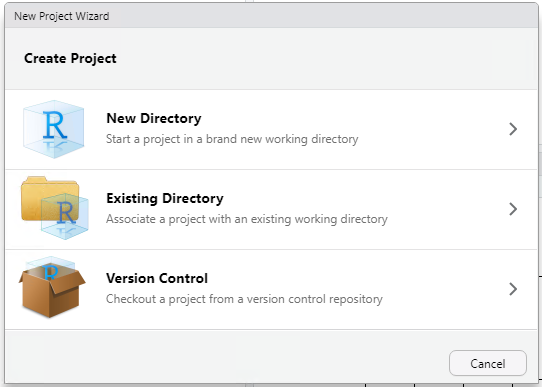
\includegraphics[width=7.53in]{images/chapter1/rstudio_6} \caption{RStudio Desktop. Новий проект}\label{fig:unnamed-chunk-17}
\end{figure}

На наступному кроці обираємо \texttt{New\ Project}:

\begin{figure}
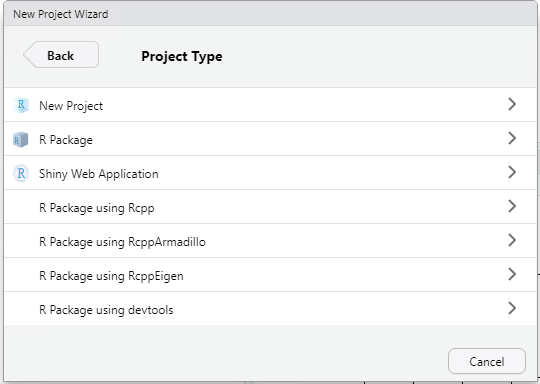
\includegraphics[width=7.5in]{images/chapter1/rstudio_7} \caption{RStudio Desktop. Новий проект. Тип проекту}\label{fig:unnamed-chunk-18}
\end{figure}

Після кліку на \texttt{Create\ Project} буде створено папку за попередньо обраним шляхом. Для запуску проекту або швидкого перемикання між проектами можна скористатися як пунктами головного меню, так і підменю проектів справа. Також відкрити проект можна запуском файлу \texttt{*.Rproj} у провіднику \texttt{Windows}.

\begin{figure}
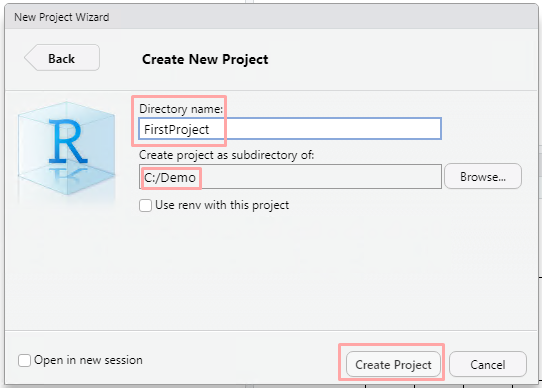
\includegraphics[width=7.53in]{images/chapter1/rstudio_8} \caption{RStudio Desktop. Новий проект}\label{fig:unnamed-chunk-19}
\end{figure}

Щоб додати новий файл з кодом \texttt{R} потрібно обрати з головного меню \texttt{File\ \textgreater{}\ New\ file\ \textgreater{}\ R\ Script} або скористатися командою \texttt{Ctrl+Shift+N}. Новий файл буде створено з назвою \texttt{Untitled{[}X{]}}, тому рекомендую одразу його зберегти, наприклад, як \texttt{TestCode.R}

Для першого проекту розвяжемо наступну задачу:

\begin{quote}
Написати програму, що генерує вектор з 20-ти випадкових чисел у межах {[}1;5{]}, обчислює середнє та суму чисел, а також виводить гістограму частоти кожного значення (скільки разів дане число повторюється у векторі).
\end{quote}

Код для генерації 20-ти випадкових чесел у діапазоні {[}1;5{]} матиме наступний вигляд:

\begin{Shaded}
\begin{Highlighting}[]
\NormalTok{vtr }\OtherTok{\textless{}{-}} \FunctionTok{sample}\NormalTok{(}\DecValTok{1}\SpecialCharTok{:}\DecValTok{5}\NormalTok{, }\DecValTok{20}\NormalTok{, }\AttributeTok{replace=}\ConstantTok{TRUE}\NormalTok{)}
\NormalTok{vtr}
\end{Highlighting}
\end{Shaded}

\begin{verbatim}
##  [1] 2 5 5 4 2 4 1 1 1 2 3 5 3 3 3 5 2 2 2 3
\end{verbatim}

Результати виконання на Вашому ПК будуть іншими, адже \textbf{псевдо}генератор випадкових чисел буде брати іншу ``точку відліку'' для генерування чисел. Рекомендую перегляду функцію \texttt{set.seed(точка\ відліку\ -\ число)}.

\emph{P.S. Також зустрічав у мережі інформацію, що робота \texttt{set.seed()} для \texttt{R} у \texttt{4+} версії може відрізнятися від \texttt{3+}. Після перевірки інформації оновлю даний текст.}

Обчислення та виведення на консоль інформації про суму та середнє значення:

\begin{Shaded}
\begin{Highlighting}[]
\NormalTok{vtr\_sum }\OtherTok{\textless{}{-}} \FunctionTok{sum}\NormalTok{(vtr)}
\NormalTok{vtr\_mean }\OtherTok{\textless{}{-}} \FunctionTok{mean}\NormalTok{(vtr)}

\FunctionTok{print}\NormalTok{(}\FunctionTok{paste0}\NormalTok{(}\StringTok{"Sum: "}\NormalTok{, vtr\_sum))}
\end{Highlighting}
\end{Shaded}

\begin{verbatim}
## [1] "Sum: 58"
\end{verbatim}

\begin{Shaded}
\begin{Highlighting}[]
\FunctionTok{print}\NormalTok{(}\FunctionTok{paste0}\NormalTok{(}\StringTok{"Mean: "}\NormalTok{, vtr\_mean))}
\end{Highlighting}
\end{Shaded}

\begin{verbatim}
## [1] "Mean: 2.9"
\end{verbatim}

Виведемо гістограму:

\begin{Shaded}
\begin{Highlighting}[]
\FunctionTok{hist}\NormalTok{(vtr, }\AttributeTok{breaks =} \DecValTok{5}\NormalTok{)}
\end{Highlighting}
\end{Shaded}

\begin{figure}
\centering
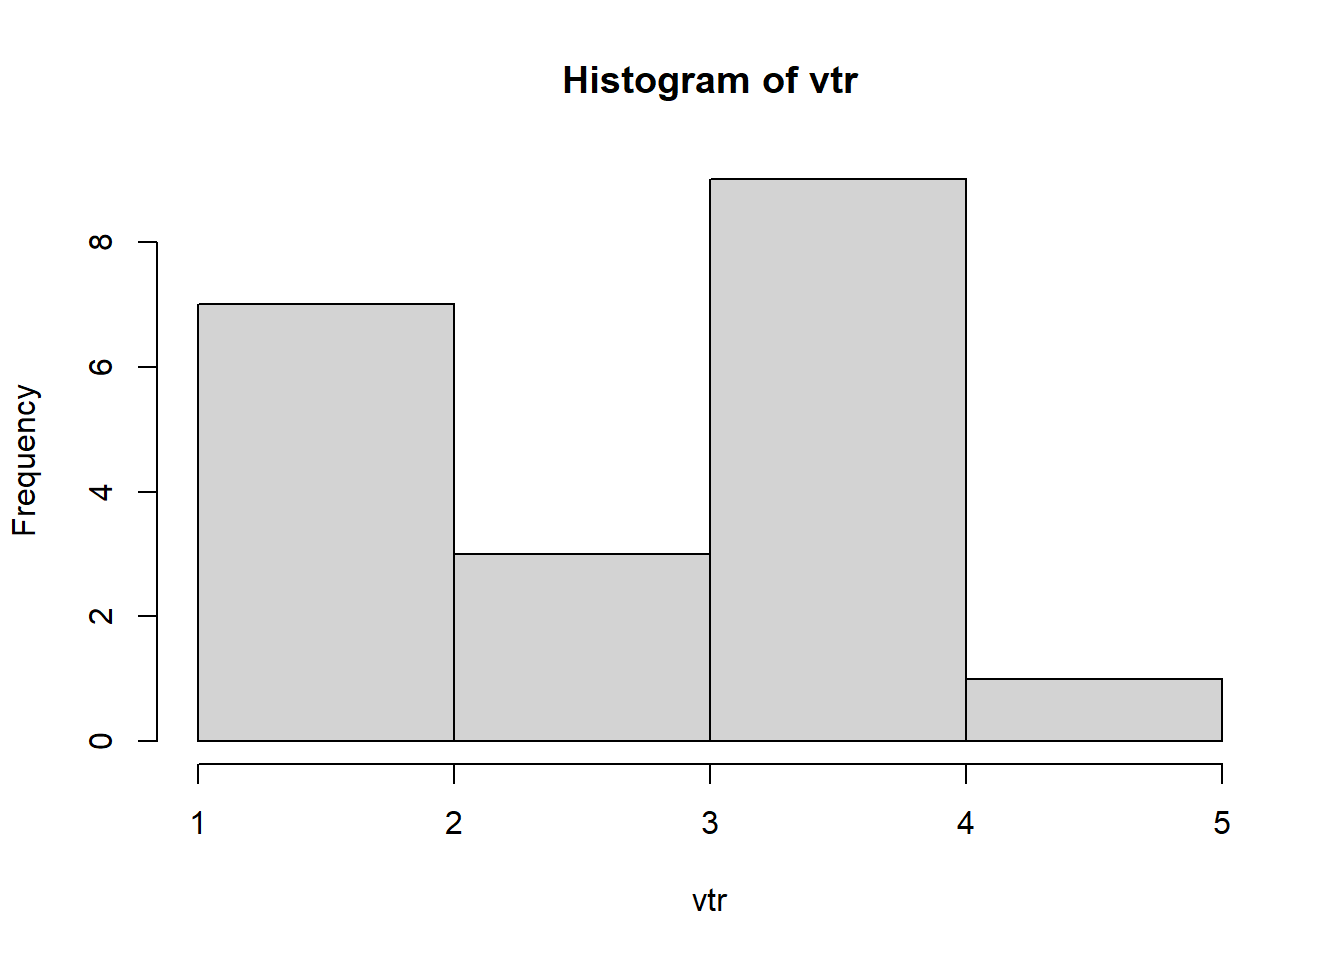
\includegraphics{01-chapter1_files/figure-latex/unnamed-chunk-22-1.pdf}
\caption{\label{fig:unnamed-chunk-22}Приклад візуалізації гістрограми в R}
\end{figure}

\emph{Примітка. Детальніше про параметри функції \texttt{hist()} можна почитати тут: \url{https://www.rdocumentation.org/packages/graphics/versions/3.6.2/topics/hist}}.

Орієнтовний вигляд вікна \texttt{RStudio} після викоання усіх описаних вище операцій матиме настпуний вигляд:

\begin{figure}
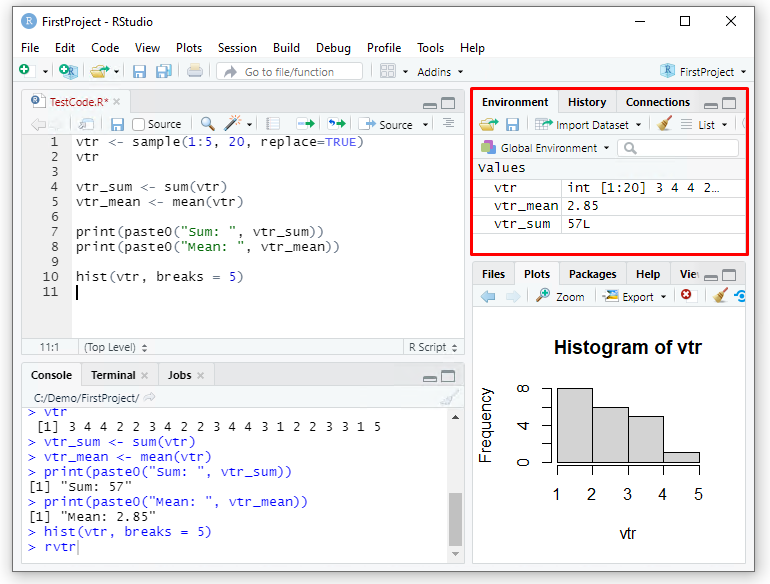
\includegraphics[width=10.69in]{images/chapter1/rstudio_10} \caption{RStudio Desktop. Перегляд змінних}\label{fig:unnamed-chunk-23}
\end{figure}

Варто звернути увагу на виділений блок \texttt{Environment}, де можна переглянути усі доступні змінні, що є на даний момент у \texttt{пам\textquotesingle{}яті}. До цих параметрів можна звертатися у коді чи з консолі у будь, який момент. \emph{Детальну інформацію про робоче середовище розглянуто нижче.}

\hypertarget{chapter133}{%
\subsection{Робота з Jupyter Notebook}\label{chapter133}}

Ноутбуки стали зручним та поширеним інструментом для аналізу даних, а також послідовного викладення матеріалів чи результатів дослідження. Перевагою такого інструменту є перемішування коду, результатів його виконання та іншого текстового наповнення, що дозволяє сформувати ``на льоту'' готові до читання документи.

\_*Примітка. Лекційні матеріали даного курсу виконані саме у ноутбуках.\_

Використання ноутбуків у навчальному процесі дозволяє описати не лише теоретичний матеріал, але приклади коду, що будуть виконувати безпосередньо під час ознайомлення з лекцією. Також слухач курсу може відредагувати наявний код та перевірити результати його виконання.

Розгялнемо процес інсталяції та запуску \texttt{Anaconda} (середовище з відкритим кодом для вирішення задач \texttt{Data\ Science}) та \texttt{Jupyter\ Notebook} на ПК.

Для встановлення середовища \texttt{Anaconda} потрібно перейти на сайт проекту та завантажити індивідуальну версію продукту: \url{https://www.anaconda.com/products/individual} \citep{Anaconda-site}.

\_*Примітка. Усі операції у даному курсі виконуються під операційну систему \texttt{Windows\ 10\ Education}\_.

Процес інсталяції середовища Anaconda не відрізняється від стандарного покрокового вставнолення програм у \texttt{Windows}.

Після запуску \texttt{Anaconda\ Navigator} для початку потрібно створити нове середовище та налаштувати роботу \texttt{R}:

\begin{figure}
\centering

\includegraphics{images/chapter1/anaconda_1.png}
\caption{Anaconda}
\end{figure}

Для початку потрібно перейти на вкладку \texttt{Environments} та натиснути \texttt{Create}:

\begin{figure}
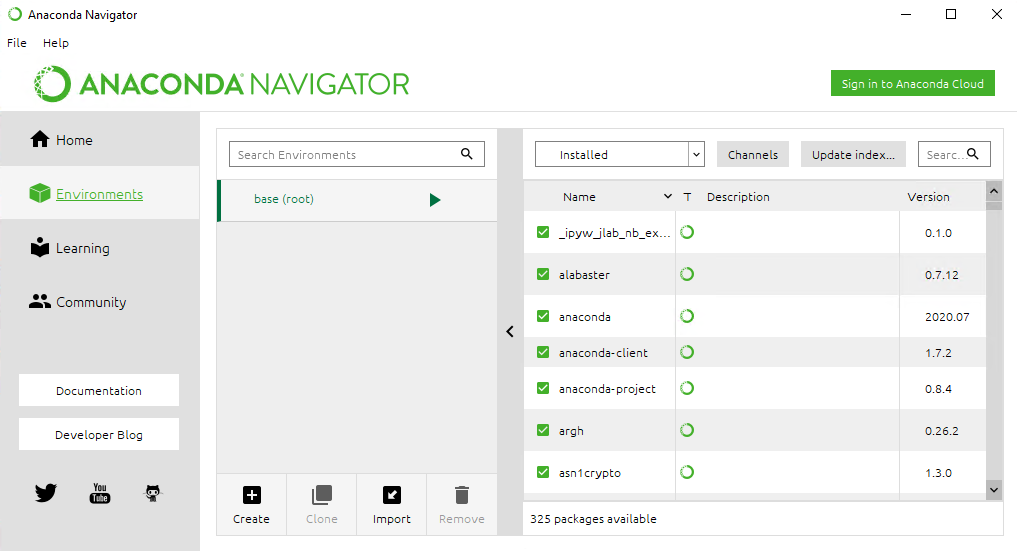
\includegraphics[width=14.12in]{images/chapter1/anaconda_2} \caption{Anaconda. Головне вікно}\label{fig:unnamed-chunk-24}
\end{figure}

У вікні, що відкрилося потрібно відмітити {[}x{]} вставновлення інструментів для роботи з \texttt{R}:

\begin{figure}
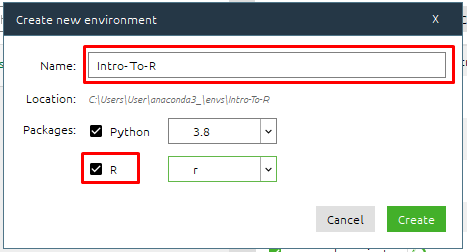
\includegraphics[width=6.49in]{images/chapter1/anaconda_3} \caption{Anaconda. Створення нового середовища на основі R}\label{fig:unnamed-chunk-25}
\end{figure}

Після встановлення R-інструментів оптрібно переключитися на вкладку \texttt{Home} та робочий простір:

\begin{figure}
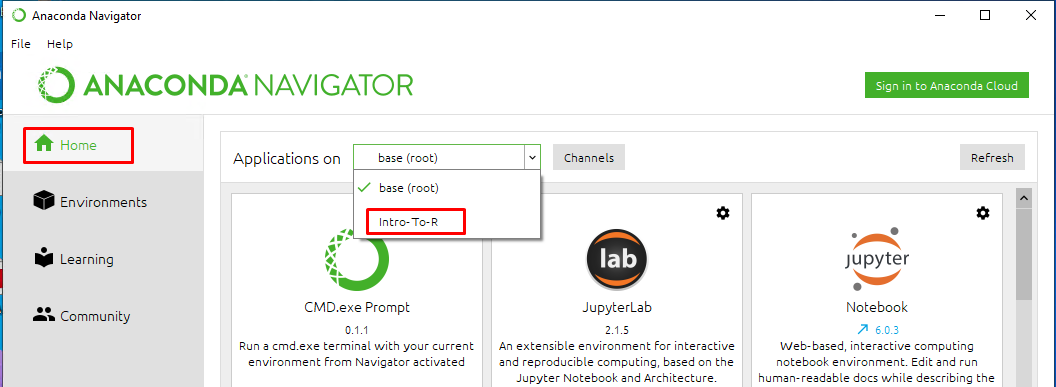
\includegraphics[width=14.67in]{images/chapter1/anaconda_4} \caption{Anaconda. Зміна середовища}\label{fig:unnamed-chunk-26}
\end{figure}

Після завантаження робочого простору оберіть \texttt{Launch} для запуску \texttt{Jupyter\ Notebook} з переліку встановлених засобів. \texttt{Jupyter\ Notebook} буде запущено у браузері за замовчеванням Вашого ПК. Відкрити ноутбук можна обравши потрібний файл, а створити новий у меню справа \texttt{New} \textgreater{} \texttt{Notebook} \textgreater{} \texttt{R}:

\begin{figure}
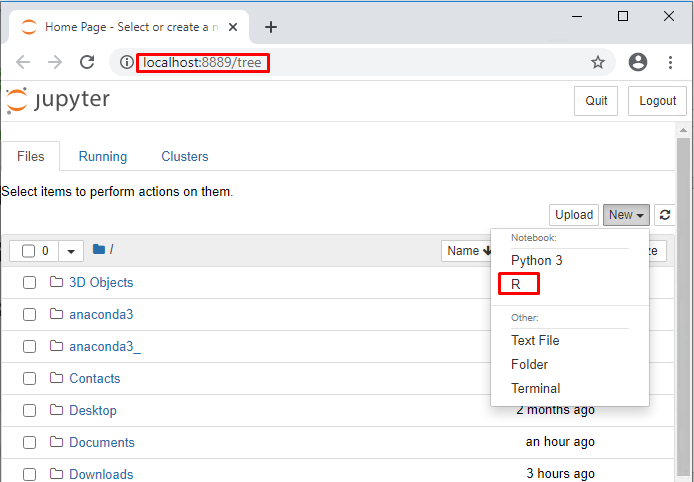
\includegraphics[width=9.64in]{images/chapter1/anaconda_6} \caption{Jupyter Notebook. Створення нового ноутбука}\label{fig:unnamed-chunk-27}
\end{figure}

\hypertarget{chapter134}{%
\subsection{Огляд додаткових IDE та сервісів для роботи з R}\label{chapter134}}

Окрім середовищ описаних вище існує ряд досить цікавих інструментів, що роблять досить зручною роботу з \texttt{R}-кодом. Розглянемо ці інструменти.

\textbf{Visual Studio Code} - безкоштовний редактор коду від \texttt{Microsoft}, орієнтовний на велику кількість мов програмування та фреймворків \citep{vs-code}. Серед інших іструментів у VS Code доступні також розширення для роботи з \texttt{R}:

\begin{figure}
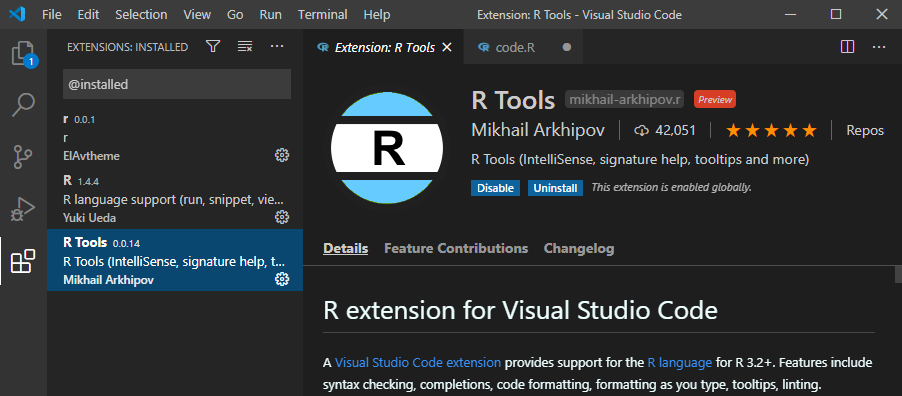
\includegraphics[width=12.53in]{images/chapter1/vs_code} \caption{Visual Studio Code. Інсталяція RTools}\label{fig:unnamed-chunk-28}
\end{figure}

\textbf{Visual Studio Community Edition} - безкоштовне середовище розробки від компаній Microsoft. VS створено з самого початку для розробки під платформу .NET та мови програмування C\#, VB.NET, F\# тощо, але з часом отримало багато розширень, що дозволяють у тому числі, працювати і з проектами в \texttt{R} \citep{visual-studio}.

\textbf{Google Collab} - онлайн сервіс для роботи з ноутбуками для \texttt{Data\ Science} від компанії \texttt{Google} \citep{google-collab}:

\begin{figure}
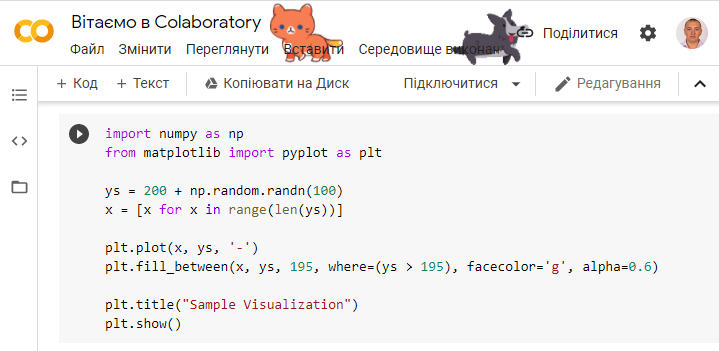
\includegraphics[width=9.99in]{images/chapter1/google_collab} \caption{Google Collab}\label{fig:unnamed-chunk-29}
\end{figure}

\emph{Примітка. Код у прикладі вище написаний на \texttt{Python}.}

\href{https://kaggle.com}{\textbf{kaggle.com}} - сервіс для змагань з \texttt{Data\ Science} та \texttt{Machine\ Learning}. Окрім переліку змагань, наборів даних сервіс має досить зручні ноутбуки.

\begin{figure}
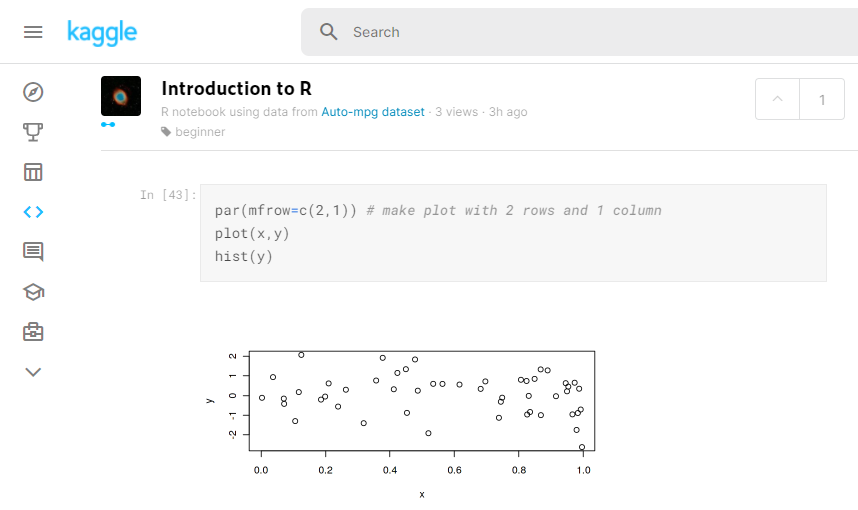
\includegraphics[width=11.92in]{images/chapter1/kaggle} \caption{Kaggle.com}\label{fig:unnamed-chunk-30}
\end{figure}

Загалом сервісів та середовищ для розробки в \texttt{R} існує досить багато і їх кількість зростає, але це не впливає на принципи написання коду та роботу з даними.

\begin{center}\rule{0.5\linewidth}{0.5pt}\end{center}

\hypertarget{chapter14}{%
\section{Основи роботи з пакетами в R}\label{chapter14}}

\hypertarget{chapter141}{%
\subsection{Команди для роботи з пакетами}\label{chapter141}}

Своєю популярністю \texttt{R} завдячує, у тому числі, і можливості швидко реалізувати досить складні дослідження за допомогою наборів уже готових функції. Такі функції обєднуються у пакети та публікуються вченими, досліджниками та розробниками зі всього світу.

\textbf{Пакети в R} - організовані набори методів та класів для виконання вузького набору задач під час програмування на \texttt{R}. Вони містять як функції так і опис способів їх використання, а чтакож дані для відтворення прикладів коду.

Пакети можуть бути завантажені з офіційного сайту проекту \href{https://cran.r-project.org/web/packages/available_packages_by_name.html}{cran.r-project.org} / \citep{R-base} або інших джерел (dev-версії є доступні на \texttt{github}). Завантаження пакетів у \texttt{R} можна здійснювати як з локального диска, так і з серверів у мережі інтернет.

Для встановлення пакету використовується команда \textbf{\texttt{install.packages()}}:

\begin{Shaded}
\begin{Highlighting}[]
\FunctionTok{install.packages}\NormalTok{(}\StringTok{"fun"}\NormalTok{)}
\end{Highlighting}
\end{Shaded}

Для підключення пакету та його використання варто скористатися \texttt{library()}:

\begin{Shaded}
\begin{Highlighting}[]
\FunctionTok{packageDescription}\NormalTok{(}\StringTok{"fun"}\NormalTok{)}
\FunctionTok{help}\NormalTok{(}\AttributeTok{package =} \StringTok{"fun"}\NormalTok{)}
\end{Highlighting}
\end{Shaded}

Дуже рекомендую почитати детальніше про пакети у статті на \texttt{DataCamp}:
R Packages: A Beginner's Guide.

\hypertarget{chapter142}{%
\subsection{Робота з пакетами в RStudio}\label{chapter142}}

Робота з пакетами в RStudio організована досить зручно і дозволяє швидко переглянути інформацію про пакет та функції, які він дозволяє використати.

Для інсталяції та оновлення пакетів можна скористатися меню \texttt{Tools}:

\begin{figure}
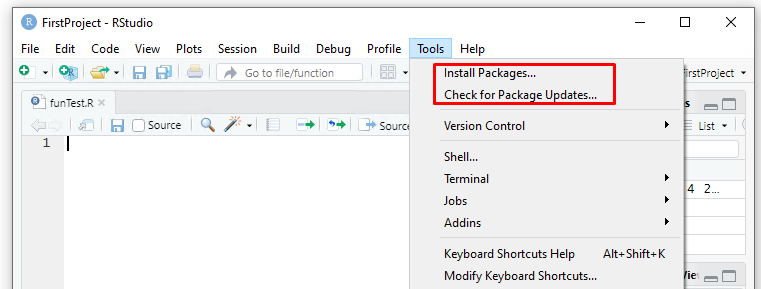
\includegraphics[width=10.57in]{images/chapter1/packages_1} \caption{RStudio Desktop. Меню інсталяції пакетів}\label{fig:unnamed-chunk-31}
\end{figure}

Після вибору \texttt{Install\ Packages...} відкриється вікно, де можна обрати як джерело інсталяції пакету так і сам пакет з переліку, ввівши кілька перших букв його назви:

\begin{figure}
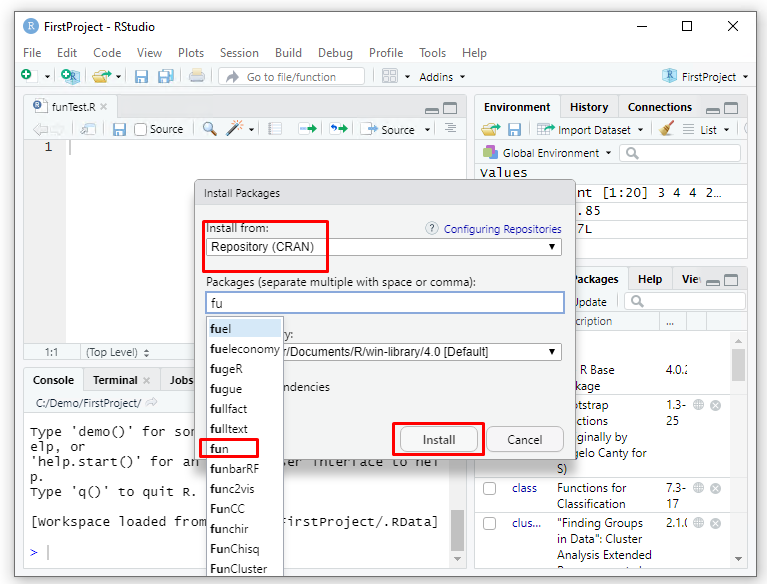
\includegraphics[width=10.65in]{images/chapter1/packages_2} \caption{RStudio Desktop. Вибір пакету для інсталяції}\label{fig:unnamed-chunk-32}
\end{figure}

\texttt{RStudio} дозволяє також переглянути інстальовані пакети/бібліотеки, розроблені іншими користувачами та завантажені у пам'ять (``галочка'' навпроти назви пакету):

\begin{figure}
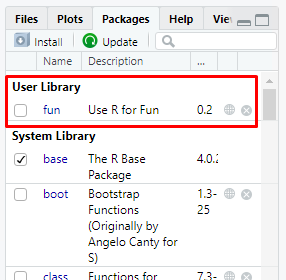
\includegraphics[width=3.97in]{images/chapter1/packages_3} \caption{RStudio Desktop. Перегляд інстальованих пакетів}\label{fig:unnamed-chunk-33}
\end{figure}

Доступ до функцій та інших елементів пакету можна здійснювати використавши запис \texttt{назва\_пакету::назва\_функції()} без підключення бібліотеки за допомогою \texttt{library()}:

\begin{figure}
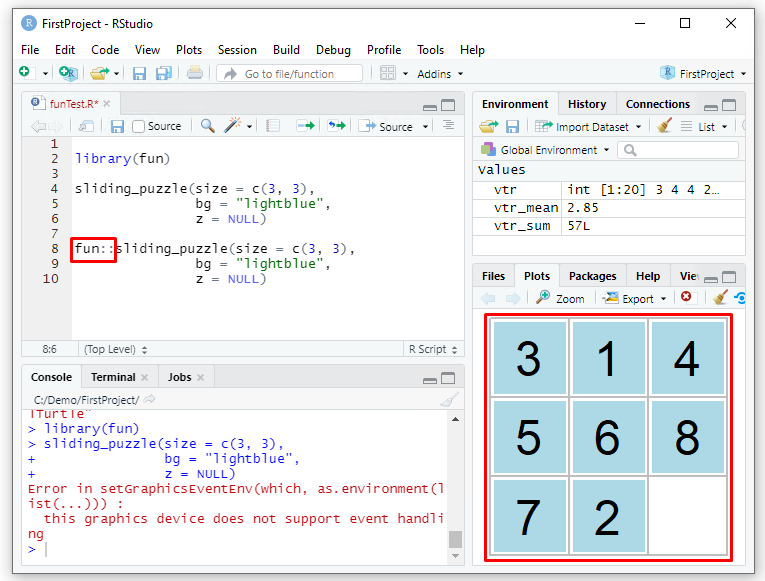
\includegraphics[width=10.62in]{images/chapter1/packages_4} \caption{RStudio Desktop. Приклад використання пакету `fun`}\label{fig:unnamed-chunk-34}
\end{figure}

Користувачі можуть не тільки завантажувати існуючі пакети,але істворювати власні та роботи їх доступними для дослідників зі всього світу.

\hypertarget{chapter2}{%
\chapter{Базові конструкції мови R}\label{chapter2}}

\hypertarget{ux43fux43bux430ux43d-1}{%
\section*{План}\label{ux43fux43bux430ux43d-1}}
\addcontentsline{toc}{section}{План}

\begin{itemize}
\tightlist
\item
  \protect\hyperlink{chapter21}{Оголошення та ініціалізація змінних}

  \begin{itemize}
  \tightlist
  \item
    \protect\hyperlink{chapter211}{Поняття змінних та оператор присвоєння}
  \item
    \protect\hyperlink{chapter212}{Правила іменування змінних}
  \end{itemize}
\item
  \protect\hyperlink{chapter22}{Базові типи даних}

  \begin{itemize}
  \tightlist
  \item
    \protect\hyperlink{chapter221}{Типізація в R}
  \item
    \protect\hyperlink{chapter222}{Перевірка та привдення типів даних}
  \end{itemize}
\item
  \protect\hyperlink{chapter23}{Оператори}

  \begin{itemize}
  \tightlist
  \item
    \protect\hyperlink{chapter231}{Арифметичні оператори}
  \item
    \protect\hyperlink{chapter232}{Оператори відношення}
  \item
    \protect\hyperlink{chapter233}{Логічні оператори}
  \end{itemize}
\item
  \protect\hyperlink{chapter24}{Корисні математичні функції}

  \begin{itemize}
  \item
    \protect\hyperlink{chapter241}{Заокруглення чисел(round, ceiling, floor, trunc, signif)}
  \item
    \protect\hyperlink{chapter242}{Послідовності чисел (seq, rep)}
  \item
    \protect\hyperlink{chapter243}{Генерація псевдовипадкових чисел}
  \item
    \protect\hyperlink{chapter244}{Інші математичні функції та константи R}
  \item ~
    \hypertarget{ux432ux432ux435ux434ux435ux43dux43dux44f-ux432ux438ux432ux435ux434ux43dux43dux44f-ux434ux430ux43dux438ux445}{%
    \section{\texorpdfstring{\protect\hyperlink{chapter245}{Введення-виведння даних}}{Введення-виведння даних}}\label{ux432ux432ux435ux434ux435ux43dux43dux44f-ux432ux438ux432ux435ux434ux43dux43dux44f-ux434ux430ux43dux438ux445}}
  \end{itemize}
\end{itemize}

\hypertarget{chapter21}{%
\section{Оголошення та ініціалізація змінних}\label{chapter21}}

\hypertarget{chapter211}{%
\subsection{Поняття змінних та оператор присвоєння}\label{chapter211}}

Базовим поняттям практично усіх мов програмування є \textbf{змінна}. Змінна дозволяє записати значення або об'єкт та назвати його для подальшого доступу, зміни, видалення по імені.

Наприклад, присвоєння змінній \texttt{my\_variable} значення \texttt{10} записується так: \texttt{my\_variable\ \textless{}-\ 5} або \texttt{my\_variable\ =\ 5}.

Операція надання змінній певного значення у програмуванні називається \textbf{присвоєнням}.

\emph{Важливо! Зверніть увагу, що присвоєння (\texttt{\textless{}-}, \texttt{=}) та рівність (\texttt{==}) це різні поняття. Оператор \texttt{==} здіснює перевірку співпадіння значення двох змінних/об'єктів та повертає результат у вигляді логічного значення \texttt{TRUE} (якщо значення рівні) або \texttt{FALSE} (якщо значення не рівні)}.

Знак \texttt{\textless{}-} не є часто використовуваним у різних мовах програмування, зазвичай для присвоєння користуються \texttt{=}. Проте в R освновним способом засобом початкової ініціалізації змінних є \texttt{\textless{}-}.

\emph{Також у програмуванні на R використовуються оператори присвоєння \texttt{\textless{}\textless{}-}, \texttt{-\textgreater{}}, \texttt{-\textgreater{}\textgreater{}}. Про них можна прочитати за лыками нижче.}

Рекомендую почитати про різницю між операторами присвоєння у R \textless- та = тут:

\begin{enumerate}
\def\labelenumi{\arabic{enumi}.}
\tightlist
\item
  \href{https://colinfay.me/r-assignment/}{Why do we use arrow as an assignment operator? (Colin FAY)}.
\item
  \href{https://renkun.me/2014/01/28/difference-between-assignment-operators-in-r/}{Difference between assignment operators in R (Ren Kun)}.
\item
  \href{https://stat.ethz.ch/R-manual/R-devel/library/base/html/assignOps.html}{Assignment Operators}.
\end{enumerate}

Приклад:

\begin{Shaded}
\begin{Highlighting}[]
\NormalTok{x }\OtherTok{\textless{}{-}} \DecValTok{45}
\NormalTok{y }\OtherTok{\textless{}{-}} \DecValTok{10}
\NormalTok{z }\OtherTok{\textless{}{-}}\NormalTok{ x }\SpecialCharTok{+}\NormalTok{ y }\CommentTok{\# z = 45 + 10}
\NormalTok{z}
\end{Highlighting}
\end{Shaded}

\begin{verbatim}
## [1] 55
\end{verbatim}

Розберемо приклад, описаний вище:

\begin{itemize}
\tightlist
\item
  У першому рядку оголошується змінна \texttt{x} і їй присвоюється значення \texttt{45}.
\item
  У другому рядку оголошується змінна \texttt{y} і їй присвоюється значення \texttt{10}.
\item
  У третьому рядку оголошується змінна \texttt{z} і їй присвоюється значення суми \texttt{x} + \texttt{y}.
  \texttt{\#} у R використовується як коментар коду, текст написаний після нього ігнорується.
\item
  У четвертому рядку відбувається виведення на консоль змінної \texttt{z}.
\end{itemize}

\hypertarget{chapter212}{%
\subsection{Правила іменування змінних}\label{chapter212}}

Є кілька основних правил іменування змінних у R:
1. Ім'я змінної може складатися з \textbf{букв} {[}a-z, A-z{]}, \textbf{цифр} {[}0-9{]}, \textbf{крапки} \texttt{.} та нижнього \textbf{підкреслювання} \texttt{\_}.
2. Ім'я змінної повинно починатися з \textbf{букви або крапки}. Якщо воно починається з крапки, то наступним символом повинна бути буква.
3. Не можна використовувати зарезервовані ключові слова мови програмування для іменування змінних, наприклад, \texttt{TRUE}/\texttt{FALSE}.

Ім'я змінної не може містити пробіл (\texttt{space}). Якщо є потреба назвати об'єкт кількома словами, то їх зазвичай розділяють підкресленням \texttt{\_} або крапкою \texttt{.}. Наприклад, змінну можна назвати \texttt{my\_variable\_name} або \texttt{my.variable.name}. Назва \texttt{myVariableName} (\href{https://en.wikipedia.org/wiki/Camel_case}{camel case}) теж буде коректно сприйнята мовою програмування R, проте такий запис тут вживається не часто.

{Приклад коректного іменування змінних:} \texttt{total}, \texttt{zminna}, \texttt{Sum}, \texttt{.length\_of\_something}, \texttt{Number123,\ x\_1}.

{Приклад неправильного іменування змінних:} \texttt{tot@l}, \texttt{5x\_1}, \texttt{\_variable}, \texttt{FALSE}, \texttt{.0ne}.

\hypertarget{chapter22}{%
\section{Базові типи даних}\label{chapter22}}

\hypertarget{chapter221}{%
\subsection{Типізація в R}\label{chapter221}}

Усі мови програмування мають власну типізацію даних з якими працюють. Тип даних - це набір властивостей певних об'єктів та операцій, що можна з ними виконувати. Так, наприклад, з \textbf{цілими числами} можна виконувати арифметичні операції додавання, віднімання та інші. Набори символів (простими словами \textbf{текст}) зазвичай можуть використовуватися для пошуку у них елементів, редагування (шляхом видалення частини існуючого або додавання нового тексту), склеювання та розділення на частини.

У \texttt{R}, на відміну від строго типізованих мов програмування, тип даних визначається на основі поточного значення елемента і може змінюватися у процесі виконання.

Розгялнемо приклад коду з мови програмування \texttt{C\#} (мова родом із \texttt{C}/\texttt{Java}):

\begin{Shaded}
\begin{Highlighting}[]
\DataTypeTok{int}\NormalTok{ a = }\DecValTok{10}\NormalTok{;}
\NormalTok{a = }\StringTok{"some text"}\NormalTok{;}
\end{Highlighting}
\end{Shaded}

Подібний код у \texttt{C\#} передбачає створення нової змінної \texttt{a} типу \texttt{int} (\texttt{integer} - ціле число), а потім відбувається присвоєння для \texttt{a} текстового фрагмента (тип \texttt{string} у \texttt{С\#}). Такий код не буде запущено і виникне {\textbf{помилка компіляції}}.

Розглянемо приклад коду з \texttt{R}:

\begin{Shaded}
\begin{Highlighting}[]
\NormalTok{a }\OtherTok{\textless{}{-}} \DecValTok{10}
\NormalTok{a }\OtherTok{\textless{}{-}} \StringTok{"some text"}
\NormalTok{a}
\end{Highlighting}
\end{Shaded}

\begin{verbatim}
## [1] "some text"
\end{verbatim}

Такий код виконається і на консоль буде виведено \texttt{some\ text}, адже у 1 першому рядку було присвоєно ціле число, у другому - текст. Таким чином \texttt{R} має \textbf{динамічну типізацію}, що дозволяє у ту ж саму змінну записати значення різних типів. Проте варто пам'ятати, що попереднє значення буде втрачено.

До базових типів даних у R варто віднести:

\begin{itemize}
\tightlist
\item
  Числа з дробовою частиною (\texttt{decimal\ numbers}), як наприклад, \texttt{4.0}, \texttt{15.214}, що називаються \textbf{\texttt{numeric(s)}}.
\item
  Натуральні числа (\texttt{natural\ numbers}), як наприклад, \texttt{4}, \texttt{15}, що називаються \textbf{\texttt{integer(s)}}.
\item
  Логічні значення (\texttt{boolean\ values}), тобто \texttt{TRUE} та \texttt{FALSE} (які також можна скорочено записувати \texttt{T} та \texttt{F}), що називаються \textbf{\texttt{logical}}.
\item
  Текст або рядки (\texttt{string\ values}), як наприклад, \texttt{"Hello"}, \texttt{"12\ is\ number"}, що називаються \textbf{\texttt{character(s)}}.
\end{itemize}

Оголосимо для прикладу три змінні: \texttt{my\_numeric} - число, \texttt{my\_character} - текст, \texttt{my\_logical} - логічне значення.

\begin{Shaded}
\begin{Highlighting}[]
\NormalTok{my\_numeric }\OtherTok{\textless{}{-}} \DecValTok{5}
\NormalTok{my\_character }\OtherTok{\textless{}{-}} \StringTok{"universe"}
\NormalTok{my\_logical }\OtherTok{\textless{}{-}} \ConstantTok{FALSE}
\end{Highlighting}
\end{Shaded}

Замінимо значення \texttt{my\_character\ \textless{}-\ "5"} та спробуємо знайти суму значень:

\begin{Shaded}
\begin{Highlighting}[]
\NormalTok{my\_character }\OtherTok{\textless{}{-}} \StringTok{"5"}
\NormalTok{my\_sum }\OtherTok{\textless{}{-}}\NormalTok{ my\_numeric }\SpecialCharTok{+}\NormalTok{ my\_character}
\end{Highlighting}
\end{Shaded}

У результаті виклання даного коду ми отримаємо помилку, адже значення \texttt{5} та \texttt{"5"} є елементами різних типів даних, перевіримо типи за допомогю функції \texttt{class()}:

\begin{Shaded}
\begin{Highlighting}[]
\FunctionTok{class}\NormalTok{(}\DecValTok{5}\NormalTok{)}
\end{Highlighting}
\end{Shaded}

\begin{verbatim}
## [1] "numeric"
\end{verbatim}

\begin{Shaded}
\begin{Highlighting}[]
\FunctionTok{class}\NormalTok{(}\StringTok{"5"}\NormalTok{)}
\end{Highlighting}
\end{Shaded}

\begin{verbatim}
## [1] "character"
\end{verbatim}

Виконання коду \texttt{class(5)} показує нам, що \texttt{5}є значенням числового типу даних \texttt{numeric}, а \texttt{class("5")} відповідає тексту \texttt{character}, тому арифметична операція додавання між цими значеннями неможлива.

\hypertarget{chapter222}{%
\subsection{Перевірка та привдення типів даних}\label{chapter222}}

У випадку коли тип даних потрібно визначити у процесі виконання програми/коду та перетворити значення використовується приведння типів даних.

\emph{Приведення типів даних} - операція перетворення значення з одного типу даних в інший. Важливо памятати, що не завжди приведення типів даних може бути здійснено. Так, наприклад, значення \texttt{"5"} (\texttt{character}) можна досить просто привести до \texttt{5} (\texttt{numeric}), проте \texttt{"five"} не буде зрозумілим для інтерпритатора.

Для перевірки належності елемента до певного типу даних використовують спеціальну функцію \texttt{is.назва\_типу(значення)}. Ця функція повертає \texttt{TRUE}, якщо елемент належить даному типу і \texttt{FALSE}, якщо не належить.

Розглянемо приклад:

\begin{Shaded}
\begin{Highlighting}[]
\NormalTok{my\_numeric }\OtherTok{\textless{}{-}} \DecValTok{5}
\NormalTok{my\_character }\OtherTok{\textless{}{-}} \StringTok{"five"}
\NormalTok{my\_logical }\OtherTok{\textless{}{-}} \ConstantTok{FALSE}

\FunctionTok{is.numeric}\NormalTok{(my\_numeric)}
\end{Highlighting}
\end{Shaded}

\begin{verbatim}
## [1] TRUE
\end{verbatim}

\begin{Shaded}
\begin{Highlighting}[]
\FunctionTok{is.character}\NormalTok{(my\_numeric)}
\end{Highlighting}
\end{Shaded}

\begin{verbatim}
## [1] FALSE
\end{verbatim}

Для перетворення типу даних можна скористатися функцією \texttt{as.назва\_типу(значення)}. У результаті виконання функції буде повернуто значення потрібного типу або пусте значення \texttt{NA}, якщо таке приведення не є можливим:

\begin{Shaded}
\begin{Highlighting}[]
\NormalTok{a }\OtherTok{\textless{}{-}} \DecValTok{5}
\NormalTok{b }\OtherTok{\textless{}{-}} \StringTok{"10"}
\NormalTok{c }\OtherTok{\textless{}{-}} \StringTok{"10, 20"}
\FunctionTok{as.numeric}\NormalTok{(b)}
\end{Highlighting}
\end{Shaded}

\begin{verbatim}
## [1] 10
\end{verbatim}

\begin{Shaded}
\begin{Highlighting}[]
\FunctionTok{as.numeric}\NormalTok{(c)}
\end{Highlighting}
\end{Shaded}

\begin{verbatim}
## Warning: NAs introduced by coercion
\end{verbatim}

\begin{verbatim}
## [1] NA
\end{verbatim}

Результат виконання функцій можна записувати у змінні і використовувати у наступних обчисленнях:

\begin{Shaded}
\begin{Highlighting}[]
\NormalTok{a }\OtherTok{\textless{}{-}} \DecValTok{5}
\NormalTok{b }\OtherTok{\textless{}{-}} \StringTok{"10"}
\NormalTok{b }\OtherTok{\textless{}{-}} \FunctionTok{as.numeric}\NormalTok{(b)}
\NormalTok{a }\SpecialCharTok{+}\NormalTok{ b}
\end{Highlighting}
\end{Shaded}

\begin{verbatim}
## [1] 15
\end{verbatim}

\begin{Shaded}
\begin{Highlighting}[]
\NormalTok{number }\OtherTok{\textless{}{-}} \FunctionTok{as.integer}\NormalTok{(}\DecValTok{54}\NormalTok{)}
\FunctionTok{typeof}\NormalTok{(number)}
\end{Highlighting}
\end{Shaded}

\begin{verbatim}
## [1] "integer"
\end{verbatim}

\begin{Shaded}
\begin{Highlighting}[]
\FunctionTok{class}\NormalTok{(number)}
\end{Highlighting}
\end{Shaded}

\begin{verbatim}
## [1] "integer"
\end{verbatim}

Повний перелік типів та методів перевірки і приведення їх типів ображений нижче:

\begin{longtable}[]{@{}lll@{}}
\toprule
Назва типу & Метод перевірки типу & Метод приведення типу\tabularnewline
\midrule
\endhead
Array & is.array & as.array\tabularnewline
\textbf{Character} & is.character & as.character\tabularnewline
Complex & is.complex & as.complex\tabularnewline
Dataframe & is.data.frame & as.data.frame\tabularnewline
\textbf{Double} & is.double & as.double\tabularnewline
Factor & is.factor & as.factor\tabularnewline
List & is.list & as.list\tabularnewline
\textbf{Logical} & is.logical & as.logical\tabularnewline
Matrix & is.matrix & as.matrix\tabularnewline
\textbf{Numeric} & is.numeric & as.numeric\tabularnewline
Raw & is.raw & as.raw\tabularnewline
Time series (ts) & is.ts & as.ts\tabularnewline
Vector & is.vector & as.vector\tabularnewline
\bottomrule
\end{longtable}

\begin{center}\rule{0.5\linewidth}{0.5pt}\end{center}

\hypertarget{chapter23}{%
\section{Оператори}\label{chapter23}}

\hypertarget{chapter231}{%
\subsection{Арифметичні оператори}\label{chapter231}}

\texttt{R} можна використовувати як звичайни калькулятор.

Розглянемо набір звичних арифметичних операторів, що відомі з початкової школи:
* Додавання: \texttt{+}.
* Віднімання: \texttt{-}.
* Ділення: \texttt{/}.
* Множення: \texttt{*}.

А також більш складні оператори:
* Піднесення до степеня: \texttt{\^{}} (вводиться з клавіатури як \texttt{Shift+6} на ENG-розкладці клавіатури).
* Остача від ділення (ще може називатися ``ділення по модулю''): \texttt{\%\%} (вводиться з клавіатури як \texttt{Shift+5}).
* Ділення націло: \texttt{\%/\%}.

Розглянемо приклад \textbf{додавання} чисел:

\begin{Shaded}
\begin{Highlighting}[]
\DecValTok{5} \SpecialCharTok{+} \DecValTok{10}
\end{Highlighting}
\end{Shaded}

\begin{verbatim}
## [1] 15
\end{verbatim}

\begin{Shaded}
\begin{Highlighting}[]
\DecValTok{5} \SpecialCharTok{+} \DecValTok{4} \SpecialCharTok{+} \DecValTok{15}
\end{Highlighting}
\end{Shaded}

\begin{verbatim}
## [1] 24
\end{verbatim}

\begin{Shaded}
\begin{Highlighting}[]
\DecValTok{5} \SpecialCharTok{+} \DecValTok{53} \SpecialCharTok{+} \DecValTok{343}
\end{Highlighting}
\end{Shaded}

\begin{verbatim}
## [1] 401
\end{verbatim}

\begin{Shaded}
\begin{Highlighting}[]
\NormalTok{(}\DecValTok{5} \SpecialCharTok{+} \DecValTok{8}\NormalTok{) }\SpecialCharTok{+}\NormalTok{ (}\DecValTok{4} \SpecialCharTok{+} \DecValTok{9}\NormalTok{)}
\end{Highlighting}
\end{Shaded}

\begin{verbatim}
## [1] 26
\end{verbatim}

\emph{Примітка}. Використання ``круглих'' дужок у прогрмуванні виразах має пріоритет аналогічний до загальноприйнятих у математиці.

Розглянемо приклад \textbf{віднімання} чисел:

\begin{Shaded}
\begin{Highlighting}[]
\DecValTok{47} \SpecialCharTok{{-}} \DecValTok{21}
\end{Highlighting}
\end{Shaded}

\begin{verbatim}
## [1] 26
\end{verbatim}

\begin{Shaded}
\begin{Highlighting}[]
\DecValTok{15} \SpecialCharTok{{-}}\NormalTok{ (}\DecValTok{10} \SpecialCharTok{{-}} \DecValTok{25}\NormalTok{)}
\end{Highlighting}
\end{Shaded}

\begin{verbatim}
## [1] 30
\end{verbatim}

\emph{Примітка}. Заміна знаків до/в ``дужках'' тут працює так само як працювала у школі :)

Приклади \textbf{множення} чисел:

\begin{Shaded}
\begin{Highlighting}[]
\DecValTok{5} \SpecialCharTok{*} \DecValTok{3}
\end{Highlighting}
\end{Shaded}

\begin{verbatim}
## [1] 15
\end{verbatim}

\begin{Shaded}
\begin{Highlighting}[]
\DecValTok{5} \SpecialCharTok{*}\NormalTok{ (}\DecValTok{2} \SpecialCharTok{+} \DecValTok{5}\NormalTok{)}
\end{Highlighting}
\end{Shaded}

\begin{verbatim}
## [1] 35
\end{verbatim}

Приклади \textbf{ділення} чисел:

\begin{Shaded}
\begin{Highlighting}[]
\DecValTok{12} \SpecialCharTok{/} \DecValTok{2}
\end{Highlighting}
\end{Shaded}

\begin{verbatim}
## [1] 6
\end{verbatim}

\begin{Shaded}
\begin{Highlighting}[]
\NormalTok{(}\DecValTok{4} \SpecialCharTok{+} \DecValTok{7}\NormalTok{) }\SpecialCharTok{/} \DecValTok{3}
\end{Highlighting}
\end{Shaded}

\begin{verbatim}
## [1] 3.666667
\end{verbatim}

\textbf{Піднесення до степеня} за допомогю оператора \texttt{\^{}} є досить простим. Так, наприклад, \texttt{3\^{}2} дорівнює 9, а \texttt{2\^{}3} - це \texttt{2*2*2} і дорівнює 8.

\begin{Shaded}
\begin{Highlighting}[]
\DecValTok{5}\SpecialCharTok{\^{}}\DecValTok{2}
\end{Highlighting}
\end{Shaded}

\begin{verbatim}
## [1] 25
\end{verbatim}

\begin{Shaded}
\begin{Highlighting}[]
\NormalTok{(}\DecValTok{1}\SpecialCharTok{+}\DecValTok{3}\NormalTok{)}\SpecialCharTok{\^{}}\DecValTok{3} \SpecialCharTok{+} \DecValTok{100} 
\end{Highlighting}
\end{Shaded}

\begin{verbatim}
## [1] 164
\end{verbatim}

\textbf{Остача від ділення} дозволяє знайти залишок одного числа від ділення на інше число.

Наприклад, остача від ділення націло 5 на 2 дорівнює 1, бо \texttt{2\ *\ 2\ (=4)\ +\ 1\ =\ 5}

\begin{Shaded}
\begin{Highlighting}[]
\DecValTok{28} \SpecialCharTok{\%\%} \DecValTok{7}
\end{Highlighting}
\end{Shaded}

\begin{verbatim}
## [1] 0
\end{verbatim}

\begin{Shaded}
\begin{Highlighting}[]
\DecValTok{17}\SpecialCharTok{\%\%}\DecValTok{5}
\end{Highlighting}
\end{Shaded}

\begin{verbatim}
## [1] 2
\end{verbatim}

\textbf{Ділння націло} залишає лише цілу частину від ідленнядвох чисел:

\begin{Shaded}
\begin{Highlighting}[]
\DecValTok{28} \SpecialCharTok{\%/\%} \DecValTok{7}
\end{Highlighting}
\end{Shaded}

\begin{verbatim}
## [1] 4
\end{verbatim}

\begin{Shaded}
\begin{Highlighting}[]
\DecValTok{17} \SpecialCharTok{\%/\%} \DecValTok{5} 
\end{Highlighting}
\end{Shaded}

\begin{verbatim}
## [1] 3
\end{verbatim}

\begin{Shaded}
\begin{Highlighting}[]
\FunctionTok{Sys.setlocale}\NormalTok{(}\StringTok{"LC\_CTYPE"}\NormalTok{, }\StringTok{"ukrainian"}\NormalTok{)}
\end{Highlighting}
\end{Shaded}

\begin{verbatim}
## [1] "Ukrainian_Ukraine.1251"
\end{verbatim}

\begin{Shaded}
\begin{Highlighting}[]
\CommentTok{\# пробіли між цифрами та операторами можна не лишати, це робиться для зручності візуального сприйняття коду}
\end{Highlighting}
\end{Shaded}

В окремих випадках інтерпритатори \texttt{R} можуть некоректно читати або взагалі ввжати за помилку наявність кирилиці у коді. Тоді варто вказати явно локалізацію, яку Ви бажаєте використовувати. Для української локалізації варто на початку коду додати рядок:

\begin{Shaded}
\begin{Highlighting}[]
\FunctionTok{Sys.setlocale}\NormalTok{(}\StringTok{"LC\_CTYPE"}\NormalTok{, }\StringTok{"ukrainian"}\NormalTok{)}
\end{Highlighting}
\end{Shaded}

\hypertarget{chapter232}{%
\subsection{Оператори відношення}\label{chapter232}}

\textbf{Оператори відношення} відповідають за порівнняння двох об'єктів між собою та повертають значення логічного типу \texttt{TRUE}, якщо результат істинний та \texttt{FALSE}, якщо результат хибний.

Перелік операторів відношення:

\begin{itemize}
\tightlist
\item
  Більше або дорівнює \texttt{\textgreater{}=}.
\item
  Менше \texttt{\textless{}}.
\item
  Менше або дорівнює \texttt{\textless{}=}.
\item
  Дорівнює \texttt{==}.
\item
  Не дорівнює \texttt{!=}
\end{itemize}

Для демонстрації принципів роботи операторів відношення оголосимо 3 змінні \texttt{a}, \texttt{b} та \texttt{c}.

\begin{Shaded}
\begin{Highlighting}[]
\NormalTok{a }\OtherTok{\textless{}{-}} \DecValTok{12}
\NormalTok{b }\OtherTok{\textless{}{-}} \DecValTok{5}
\NormalTok{c }\OtherTok{\textless{}{-}} \DecValTok{7}
\end{Highlighting}
\end{Shaded}

Розгялнемо кілька прикладів використання описаних вище операторів.

Оператори, що відповідають за первірку на ``більше/менше'':

\begin{Shaded}
\begin{Highlighting}[]
\NormalTok{a }\SpecialCharTok{\textgreater{}}\NormalTok{ b}
\end{Highlighting}
\end{Shaded}

\begin{verbatim}
## [1] TRUE
\end{verbatim}

\begin{Shaded}
\begin{Highlighting}[]
\NormalTok{b }\SpecialCharTok{+}\NormalTok{ c }\SpecialCharTok{\textless{}}\NormalTok{ a}
\end{Highlighting}
\end{Shaded}

\begin{verbatim}
## [1] FALSE
\end{verbatim}

\begin{Shaded}
\begin{Highlighting}[]
\NormalTok{b }\SpecialCharTok{+}\NormalTok{ c }\SpecialCharTok{\textless{}=}\NormalTok{ a}
\end{Highlighting}
\end{Shaded}

\begin{verbatim}
## [1] TRUE
\end{verbatim}

Оператори, що відповідають за перевірку на ``рівність/нерівність'':

\begin{Shaded}
\begin{Highlighting}[]
\NormalTok{a }\SpecialCharTok{!=}\NormalTok{ b}
\end{Highlighting}
\end{Shaded}

\begin{verbatim}
## [1] TRUE
\end{verbatim}

\begin{Shaded}
\begin{Highlighting}[]
\NormalTok{a }\SpecialCharTok{==}\NormalTok{ b }\SpecialCharTok{+}\NormalTok{ c}
\end{Highlighting}
\end{Shaded}

\begin{verbatim}
## [1] TRUE
\end{verbatim}

\begin{Shaded}
\begin{Highlighting}[]
\NormalTok{b }\SpecialCharTok{==}\NormalTok{ c}
\end{Highlighting}
\end{Shaded}

\begin{verbatim}
## [1] FALSE
\end{verbatim}

\hypertarget{chapter233}{%
\subsection{Логічні оператори}\label{chapter233}}

До логічних операторів у \texttt{R} відносяться:

\begin{itemize}
\tightlist
\item
  І \texttt{\&} (амперсант, \texttt{Shift-7}) - виконання усіх умов одночасно.
\item
  АБО \texttt{\textbar{}} (вертикальна риска, \texttt{Shift+\textbackslash{}}) - виконання однієї із умов.
\item
  НЕ \texttt{!} (знак оклику, \texttt{Shift+1}) - заперечення.
\end{itemize}

Важливо розуміти відмінності між цими операторами вміти використовувати результи їх роботи. Для початку варто розглянути таблицю істинності:

\begin{longtable}[]{@{}lllll@{}}
\toprule
A & B & Оператор \textbf{І} & Оператор \textbf{АБО} & Заперечення A (\textbf{не A})\tabularnewline
\midrule
\endhead
FALSE & FALSE & FALSE & FALSE & TRUE\tabularnewline
FALSE & TRUE & FALSE & TRUE & TRUE\tabularnewline
TRUE & FALSE & FALSE & TRUE & FALSE\tabularnewline
TRUE & TRUE & TRUE & TRUE & FALSE\tabularnewline
\bottomrule
\end{longtable}

Матеріали розділу не доповнені прикладами.

\begin{center}\rule{0.5\linewidth}{0.5pt}\end{center}

\hypertarget{chapter24}{%
\section{Корисні математичні функції}\label{chapter24}}

\hypertarget{chapter241}{%
\subsection{Заокруглення чисел (round, ceiling, floor, trunc, signif)}\label{chapter241}}

Як ми знаємо з математики, що заокруглення чисел буває ``вверх'', ``вниз'' або відносно деякого значення, зазвичай пов'язаного із цифрою \texttt{5} (\texttt{3.6} заокруглюємо до цілого як \texttt{4}, а \texttt{3.2} як \texttt{3}, ввжаючи \texttt{3.5} межею).

Увага! Заокрулення чисел у програмуванні може призводити до помилок у результатах обчислень. Для задач бізнесу або технічних процесів мінімальні відхилення можуть призводити до викривлених результатів або збоїв у системах.

\emph{\textbf{Функція \texttt{round()}}}

~ Примітка. Тут і надалі функції будуть позначатися як назва() (назва і ``круглі'' дужки).

Для заокруглення дійних чисел (з дробовою частиною) за правилом \texttt{\textless{}0.5\ \&\ \textgreater{}=0.5} (не знаю як називається науково) використовується функція \texttt{round(x,\ y)}, де \texttt{x} - число, \texttt{y} - точність (кількість знаків після коми/крапки). Наприклад:

\begin{Shaded}
\begin{Highlighting}[]
\FunctionTok{round}\NormalTok{(}\FloatTok{3.557}\NormalTok{, }\DecValTok{2}\NormalTok{)}
\end{Highlighting}
\end{Shaded}

\begin{verbatim}
## [1] 3.56
\end{verbatim}

\begin{Shaded}
\begin{Highlighting}[]
\FunctionTok{round}\NormalTok{(}\FloatTok{3.241}\NormalTok{, }\DecValTok{2}\NormalTok{)}
\end{Highlighting}
\end{Shaded}

\begin{verbatim}
## [1] 3.24
\end{verbatim}

\begin{Shaded}
\begin{Highlighting}[]
\FunctionTok{round}\NormalTok{(}\SpecialCharTok{{-}}\FloatTok{3.557}\NormalTok{, }\DecValTok{2}\NormalTok{)}
\end{Highlighting}
\end{Shaded}

\begin{verbatim}
## [1] -3.56
\end{verbatim}

\begin{Shaded}
\begin{Highlighting}[]
\FunctionTok{round}\NormalTok{(}\SpecialCharTok{{-}}\FloatTok{3.241}\NormalTok{, }\DecValTok{2}\NormalTok{)}
\end{Highlighting}
\end{Shaded}

\begin{verbatim}
## [1] -3.24
\end{verbatim}

Також можна використати \texttt{round(x)} з одним параметром, тоді заокруглення відбудеться до цілої частини, наприклад:

\begin{Shaded}
\begin{Highlighting}[]
\FunctionTok{round}\NormalTok{(}\FloatTok{124.345}\NormalTok{)}
\end{Highlighting}
\end{Shaded}

\begin{verbatim}
## [1] 124
\end{verbatim}

\emph{\textbf{Функція \texttt{floor()}}}

Для заокруглення до найближчого меншого цілого числа слід скористатися функцією \texttt{floor()}:

\begin{Shaded}
\begin{Highlighting}[]
\FunctionTok{floor}\NormalTok{(}\FloatTok{3.557}\NormalTok{)}
\end{Highlighting}
\end{Shaded}

\begin{verbatim}
## [1] 3
\end{verbatim}

\begin{Shaded}
\begin{Highlighting}[]
\FunctionTok{floor}\NormalTok{(}\FloatTok{3.241}\NormalTok{)}
\end{Highlighting}
\end{Shaded}

\begin{verbatim}
## [1] 3
\end{verbatim}

\begin{Shaded}
\begin{Highlighting}[]
\FunctionTok{floor}\NormalTok{(}\SpecialCharTok{{-}}\FloatTok{3.557}\NormalTok{)}
\end{Highlighting}
\end{Shaded}

\begin{verbatim}
## [1] -4
\end{verbatim}

\begin{Shaded}
\begin{Highlighting}[]
\FunctionTok{floor}\NormalTok{(}\SpecialCharTok{{-}}\FloatTok{3.241}\NormalTok{)}
\end{Highlighting}
\end{Shaded}

\begin{verbatim}
## [1] -4
\end{verbatim}

\emph{\textbf{Функція \texttt{ceiling()}}}

Для заокруглення до найближчого більшого цілого числа слід скористатися функцією \texttt{ceiling()}:

\begin{Shaded}
\begin{Highlighting}[]
\FunctionTok{ceiling}\NormalTok{(}\FloatTok{3.557}\NormalTok{)}
\end{Highlighting}
\end{Shaded}

\begin{verbatim}
## [1] 4
\end{verbatim}

\begin{Shaded}
\begin{Highlighting}[]
\FunctionTok{ceiling}\NormalTok{(}\FloatTok{3.241}\NormalTok{)}
\end{Highlighting}
\end{Shaded}

\begin{verbatim}
## [1] 4
\end{verbatim}

\begin{Shaded}
\begin{Highlighting}[]
\FunctionTok{ceiling}\NormalTok{(}\SpecialCharTok{{-}}\FloatTok{3.557}\NormalTok{)}
\end{Highlighting}
\end{Shaded}

\begin{verbatim}
## [1] -3
\end{verbatim}

\begin{Shaded}
\begin{Highlighting}[]
\FunctionTok{ceiling}\NormalTok{(}\SpecialCharTok{{-}}\FloatTok{3.241}\NormalTok{)}
\end{Highlighting}
\end{Shaded}

\begin{verbatim}
## [1] -3
\end{verbatim}

\emph{\textbf{Функція \texttt{trunc()}}}

Функція \texttt{trunc()} у R використовується для отримання найбільшого цілого числа, яке більше або рівне \texttt{x}. Простими словами це означає, що для чисел менших 0 \texttt{(x\ \textless{}\ 0)} \texttt{trunc()} працює як \texttt{celing()}, а для чисел більших нуля \texttt{x\ \textgreater{}\ 0}, як \texttt{floor()}:

\begin{Shaded}
\begin{Highlighting}[]
\NormalTok{x }\OtherTok{\textless{}{-}} \FloatTok{5.34}
\FunctionTok{print}\NormalTok{(}\FunctionTok{paste}\NormalTok{(}\StringTok{"trunc:"}\NormalTok{, }\FunctionTok{trunc}\NormalTok{(x), }\StringTok{"celing:"}\NormalTok{, }\FunctionTok{ceiling}\NormalTok{(x), }\StringTok{"floor:"}\NormalTok{, }\FunctionTok{floor}\NormalTok{(x), }\AttributeTok{sep =} \StringTok{" "}\NormalTok{))}
\end{Highlighting}
\end{Shaded}

\begin{verbatim}
## [1] "trunc: 5 celing: 6 floor: 5"
\end{verbatim}

\begin{Shaded}
\begin{Highlighting}[]
\NormalTok{x }\OtherTok{\textless{}{-}}\NormalTok{ x }\SpecialCharTok{*} \SpecialCharTok{{-}}\DecValTok{1}
\FunctionTok{print}\NormalTok{(}\FunctionTok{paste}\NormalTok{(}\StringTok{"trunc:"}\NormalTok{, }\FunctionTok{trunc}\NormalTok{(x), }\StringTok{"celing:"}\NormalTok{, }\FunctionTok{ceiling}\NormalTok{(x), }\StringTok{"floor:"}\NormalTok{, }\FunctionTok{floor}\NormalTok{(x), }\AttributeTok{sep =} \StringTok{" "}\NormalTok{))}
\end{Highlighting}
\end{Shaded}

\begin{verbatim}
## [1] "trunc: -5 celing: -5 floor: -6"
\end{verbatim}

\emph{\textbf{Функція \texttt{signif()}}}

Інколи виникає потреба заокруглити не десяткову частину числа, а десятки, сотні, тисячі і так далі. Розглядемо варіант, коли у нас є велике число \texttt{11\ 547\ 741.3} і нам потрібно коротко його записати як \texttt{11.5\ млн} Для таких задач можна використати функцію \texttt{signif(x,y)}, де \texttt{x} - число, яке потрібно заокруглити до певного порядку, \texttt{y} - порядок заокруглення (рахувати від початку). Наприклад:

\begin{Shaded}
\begin{Highlighting}[]
\NormalTok{big\_number }\OtherTok{\textless{}{-}} \FloatTok{11547741.3}
\NormalTok{rounded\_big\_number }\OtherTok{\textless{}{-}} \FunctionTok{signif}\NormalTok{(big\_number,}\DecValTok{3}\NormalTok{)}
\NormalTok{rounded\_big\_number}
\end{Highlighting}
\end{Shaded}

\begin{verbatim}
## [1] 11500000
\end{verbatim}

\begin{Shaded}
\begin{Highlighting}[]
\NormalTok{rounded\_big\_number }\SpecialCharTok{/} \DecValTok{1000000}
\end{Highlighting}
\end{Shaded}

\begin{verbatim}
## [1] 11.5
\end{verbatim}

\hypertarget{chapter242}{%
\subsection{Послідовності чисел (seq, rep)}\label{chapter242}}

Матеріали розділу у процесі підготовки.

\hypertarget{chapter243}{%
\subsection{Генерація псевдовипадкових чисел}\label{chapter243}}

Матеріали розділу у процесі підготовки.

\begin{Shaded}
\begin{Highlighting}[]
\FunctionTok{runif}\NormalTok{(}\DecValTok{10}\NormalTok{)}
\end{Highlighting}
\end{Shaded}

\begin{verbatim}
##  [1] 0.09125617 0.28922002 0.29474867 0.44290966 0.16358988 0.54594240
##  [7] 0.08778667 0.96161253 0.86583787 0.48742442
\end{verbatim}

\begin{Shaded}
\begin{Highlighting}[]
\FunctionTok{sample}\NormalTok{(}\DecValTok{100}\NormalTok{)}
\end{Highlighting}
\end{Shaded}

\begin{verbatim}
##   [1]  72  52  92  70  77   3   9  26  29  60  24  11  61  42  79  41  69  95
##  [19]  89  25  37   1  38   2   8  58  46  35  68  51  40  67  65  96  64  15
##  [37]  16  22  49  78  39  66  84  76  18  91  63  43   4  93  56  21  53  50
##  [55]  45  12  23 100  30  17  34  74  80   5  10  36  94  33  44  14  54  57
##  [73]  28  13   7  90  47  20  55  62  85  81   6  59  83  31  87  32  99  71
##  [91]  27  97  19  75  82  73  88  98  48  86
\end{verbatim}

\hypertarget{chapter244}{%
\subsection{Інші математичні функції та константи R}\label{chapter244}}

Окрім описаного вище набору функцій \texttt{R} містить дуже велику кількість реалізованих функцій з різних сфер науки, бізнесу, техніки тощо. Прочитати про них можна з офіційної документації пакетів, у яких вони реалізовані та знайти за допомогою функції \texttt{help()} або \texttt{?name}.

Далі розглянемо перелік найпоширеніших функцій, що використовуються для розв'язання навчальних задач під час вивчення основ програмування.

\begin{longtable}[]{@{}ll@{}}
\toprule
Функція & Призначення, опис\tabularnewline
\midrule
\endhead
\emph{log(x)} & Логарифм числа \emph{x} за основою \emph{e}\tabularnewline
\emph{log(x,n)} & Логарифм числа \emph{x} за основою \emph{n}\tabularnewline
\emph{exp(x)} & \emph{e} у степені \emph{x}\tabularnewline
\emph{sqrt(x)} & Корінь квадратний числа \emph{x}\tabularnewline
\emph{factorial(x)} & Факторіал числа \emph{x}\tabularnewline
\emph{abs(x)} & Модуль числа \emph{x}\tabularnewline
\bottomrule
\end{longtable}

Також у \texttt{R} доступні ряд тригонометричних функцій, які вивчалися у школі і не тільки, серед них \texttt{cos(x)}, \texttt{sin(x)}, \texttt{tan(x)}, а також \texttt{acos(x)}, \texttt{asin(x)}, \texttt{atan(x)}, \texttt{acosh(x)}, \texttt{asinh(x)}, \texttt{atanh(x)}.

Детальніше про кожну з них можна почитати у документації за допомогою кодманди \texttt{help(function)}.

\hypertarget{chapter245}{%
\section{Введення-виведння даних}\label{chapter245}}

Матеріали розділу у процесі підготовки.

\hypertarget{chapter3}{%
\chapter{Основи роботи з даними в R}\label{chapter3}}

\hypertarget{ux43fux43bux430ux43d-2}{%
\section*{План}\label{ux43fux43bux430ux43d-2}}
\addcontentsline{toc}{section}{План}

\begin{itemize}
\tightlist
\item
  \protect\hyperlink{chapter31}{Набори даних}
\item
  \protect\hyperlink{chapter32}{Вектори (vectors)}

  \begin{itemize}
  \tightlist
  \item
    \protect\hyperlink{chapter321}{Поняття та спосіб представлення}
  \item
    \protect\hyperlink{chapter322}{Оголошення векторів}
  \item
    \protect\hyperlink{chapter323}{Операції над векторами}
  \end{itemize}
\end{itemize}

\begin{center}\rule{0.5\linewidth}{0.5pt}\end{center}

\hypertarget{chapter31}{%
\section{Набори даних}\label{chapter31}}

Матеріали розділу у процесі підготовки.

\hypertarget{chapter32}{%
\section{Вектори (vectors)}\label{chapter32}}

\hypertarget{chapter321}{%
\subsection{Поняття та спосіб представлення}\label{chapter321}}

Вектори є найпростішим способом представлення колекції даних. З своїм змістом \textbf{вектор} - це послідовність однорідних елементів. Якщо ж говорити про мову програмування, то \textbf{вектор} - це послідовність елементів одного типу, що розміщені за деяким порядком (індексом).

Вектор прийнято позначати, як x = (x1, x2,\ldots, xn), де х - назва вектора, n - кількість елементів вектора,

\hypertarget{chapter322}{%
\subsection{Оголошення векторів}\label{chapter322}}

Вектор - базовий тип даних у \texttt{R}, що дозволяє записати колекцію елементів одного типу за допомогою \texttt{c()} або без нього, якщо це послідовність значень.

\emph{Примітка. По суті функція \texttt{c()} дозволяє об'єднати кілька векторів.}

Розглянемо для прикладу звичайну змінну \texttt{x}:

\begin{Shaded}
\begin{Highlighting}[]
\NormalTok{x }\OtherTok{\textless{}{-}} \DecValTok{10}
\end{Highlighting}
\end{Shaded}

По своїй суті \texttt{x} у даному випадку є вектором, що складається з одного значення \texttt{10}. Ми можемо також записати кілька елементів у змінну \texttt{x}:

\begin{Shaded}
\begin{Highlighting}[]
\NormalTok{x }\OtherTok{\textless{}{-}} \FunctionTok{c}\NormalTok{(}\DecValTok{1}\NormalTok{, }\DecValTok{2}\NormalTok{, }\FloatTok{2.5}\NormalTok{, }\DecValTok{3}\NormalTok{)}
\NormalTok{x}
\end{Highlighting}
\end{Shaded}

\begin{verbatim}
## [1] 1.0 2.0 2.5 3.0
\end{verbatim}

Елементами вектора можуть бути значення будь якого типу: \texttt{numeric}, \texttt{character}, \texttt{logical} тощо:

\begin{Shaded}
\begin{Highlighting}[]
\NormalTok{v1 }\OtherTok{\textless{}{-}} \FunctionTok{c}\NormalTok{(}\DecValTok{1}\NormalTok{, }\DecValTok{3}\NormalTok{, }\DecValTok{4}\NormalTok{, }\DecValTok{6}\NormalTok{, }\DecValTok{7}\NormalTok{)}
\NormalTok{v2 }\OtherTok{\textless{}{-}} \FunctionTok{c}\NormalTok{(T, F, F, T, F)}
\NormalTok{v3 }\OtherTok{\textless{}{-}} \FunctionTok{c}\NormalTok{(}\StringTok{"Hello"}\NormalTok{, }\StringTok{"my"}\NormalTok{, }\StringTok{"friend"}\NormalTok{, }\StringTok{"!"}\NormalTok{)}
\end{Highlighting}
\end{Shaded}

Елементами вектора також послідовності, створені на за допомогою функцій \texttt{rep()}, \texttt{seq()} та оператора \texttt{:}:

\begin{Shaded}
\begin{Highlighting}[]
\NormalTok{vtr }\OtherTok{\textless{}{-}}  \DecValTok{2}\SpecialCharTok{:}\DecValTok{7}
\NormalTok{vtr}
\end{Highlighting}
\end{Shaded}

\begin{verbatim}
## [1] 2 3 4 5 6 7
\end{verbatim}

\begin{Shaded}
\begin{Highlighting}[]
\NormalTok{vtr }\OtherTok{\textless{}{-}} \DecValTok{7}\SpecialCharTok{:}\DecValTok{2}
\NormalTok{vtr}
\end{Highlighting}
\end{Shaded}

\begin{verbatim}
## [1] 7 6 5 4 3 2
\end{verbatim}

Якщо є потреба об'єднати кілька векторів, скористайтеся функцією \texttt{c()}:

\begin{Shaded}
\begin{Highlighting}[]
\NormalTok{x }\OtherTok{\textless{}{-}} \DecValTok{2}\SpecialCharTok{:}\DecValTok{3}
\NormalTok{y }\OtherTok{\textless{}{-}} \FunctionTok{c}\NormalTok{(}\DecValTok{4}\NormalTok{,}\DecValTok{6}\NormalTok{,}\DecValTok{9}\NormalTok{)}
\NormalTok{z }\OtherTok{\textless{}{-}} \FunctionTok{c}\NormalTok{(x, y, }\DecValTok{10}\SpecialCharTok{:}\DecValTok{12}\NormalTok{, }\DecValTok{100}\NormalTok{)}
\NormalTok{z}
\end{Highlighting}
\end{Shaded}

\begin{verbatim}
## [1]   2   3   4   6   9  10  11  12 100
\end{verbatim}

Переглянути коротку описову статистику по вектору можна за допомогою функції \textbf{\texttt{summary()}}:

\begin{Shaded}
\begin{Highlighting}[]
\FunctionTok{summary}\NormalTok{(z)}
\end{Highlighting}
\end{Shaded}

\begin{verbatim}
##    Min. 1st Qu.  Median    Mean 3rd Qu.    Max. 
##    2.00    4.00    9.00   17.44   11.00  100.00
\end{verbatim}

\hypertarget{chapter323}{%
\subsection{Операції над векторами}\label{chapter323}}

\hypertarget{chapter6}{%
\chapter{Приклади задач та їх розв'язки}\label{chapter6}}

\begin{center}\rule{0.5\linewidth}{0.5pt}\end{center}

\begin{itemize}
\tightlist
\item
  \protect\hyperlink{chapter61}{Задачі}

  \begin{itemize}
  \tightlist
  \item
    \protect\hyperlink{chapter611}{Послідовності та вектори}
  \item
    \protect\hyperlink{chapter612}{Функції}
  \end{itemize}
\item
  \protect\hyperlink{chapter62}{Рішення задач}

  \begin{itemize}
  \tightlist
  \item
    \protect\hyperlink{chapter621}{Послідовності та вектори}
  \item
    \protect\hyperlink{chapter622}{Функції}
  \end{itemize}
\end{itemize}

\begin{center}\rule{0.5\linewidth}{0.5pt}\end{center}

\hypertarget{chapter61}{%
\section{Задачі}\label{chapter61}}

\hypertarget{chapter611}{%
\subsection{Послідовності}\label{chapter611}}

\hypertarget{task6111}{%
\subsubsection{Задача}\label{task6111}}

Написати програму, що обчислює \(y = (x+2)^2 + ln(x)\), де \(x\) число з послідовності \texttt{100,\ 105,\ 110,\ ...,\ 200}. Результат вивести у вигляді \texttt{data.fame} з колонками \(X\) та \(Y\).

\hypertarget{task6112}{%
\subsubsection{Задача}\label{task6112}}

Написати програму, що обчислює \(y = \frac{\sqrt{x+2}}{z}\), де \(x\) число з послідовності \texttt{10,\ 15,\ 20,\ ...,\ 100}, а \(z\) - випадкові значення з діапазону \texttt{{[}-10,\ 10{]}}, що відповідає кількості елементів у \(x\). Результат вивести у вигляді \texttt{data.fame} з колонками \(X\), \(Z\) та \(Y\).

\hypertarget{task6113}{%
\subsubsection{Задача}\label{task6113}}

Без використання спеціальних функцій написати програму, що сортує вектор за зростанням та спаданням. Елементи вектора є випадковими числами з діапазону \texttt{{[}10,100)}. Кількість елементів у векторі \texttt{10}.

\hypertarget{task6114}{%
\subsubsection{Задача}\label{task6114}}

Відсортувати вектор таким чином, щоб всі додатні елементи знаходилися на початку, а всі від'ємні -- вкінці, і при цьому зберігся початковий порядок елементів в обох групах. Елементи вектора є випадковими числами з діапазону \texttt{{[}-100,100{]}}. Кількість елементів у векторі \texttt{10}.

Наприклад, якщо початковий вектор \texttt{x} складається з елементів:

\begin{Shaded}
\begin{Highlighting}[]
\NormalTok{x }\OtherTok{\textless{}{-}} \FunctionTok{c}\NormalTok{(}\DecValTok{1}\NormalTok{, }\SpecialCharTok{{-}}\DecValTok{5}\NormalTok{, }\DecValTok{10}\NormalTok{, }\SpecialCharTok{{-}}\DecValTok{8}\NormalTok{, }\SpecialCharTok{{-}}\DecValTok{2}\NormalTok{, }\DecValTok{5}\NormalTok{, }\DecValTok{4}\NormalTok{, }\SpecialCharTok{{-}}\DecValTok{9}\NormalTok{)}
\end{Highlighting}
\end{Shaded}

то після ``сортування'' він матиме вигляд:

\begin{verbatim}
## [1]  1 10  5  4 -5 -8 -2 -9
\end{verbatim}

\hypertarget{task6115}{%
\subsubsection{Задача}\label{task6115}}

Задано натуральне число \(N\) (вводиться з клавіатури). Знайти суму його цифр.

\hypertarget{task6116}{%
\subsubsection{Задача}\label{task6116}}

Задано одновимірний масив. Знайти два серед його елементів, модуль різниці яких має
найменше значення.

\hypertarget{task6117}{%
\subsubsection{Задача}\label{task6117}}

Знайти найбільший спільний дільник двох натуральних чисел, використавши алгоритм
Евкліда. Алгоритм Евкліда полягає в наступному: від більшого числа віднімається менше до тих пір,
поки вони не стануть рівними; отримане в результаті число і буде найбільшим спільним дільником.

\hypertarget{task6118}{%
\subsubsection{Задача}\label{task6118}}

Знайти мінімальний елемент серед тих елементів масиву \(A\), які не є елементами масиву \(B\).

\hypertarget{task6119}{%
\subsubsection{Задача}\label{task6119}}

Написати програму, що обчислює \textbf{середнє} значення серед парних елементів вектора. Елементи вектора генеруються випадковим чином у діапазоні \([1; 10)\). Кількість елментів вектора \texttt{10}.

\hypertarget{task6120}{%
\subsubsection{Задача}\label{task6120}}

Написати програму, що знаходить середнє значення елементів вектора. Елементи вектора генеруються випадковим чином у діапазоні \([100; 200]\). Усі елменти вектора повинні бути кратними \(7\)-ми. Генерацію випадкового числа кратного \(7\)-ми винести в окрему функцію.

\hypertarget{task6121}{%
\subsubsection{Задача}\label{task6121}}

Написати програму, що знаходить різницю між максимальним та мінімальним значенням елементів вектора, не використовуючи функції \texttt{min()} та \texttt{max()}. Елементи вектора генеруються випадковим чином у діапазоні \([10;50]\).

\hypertarget{task61211}{%
\subsubsection{Задача}\label{task61211}}

Написати програму, що знаходить різницю між максимальним та мінімальним значенням елементів вектора, не використовуючи функції \texttt{min()} та \texttt{max()}. Елементи вектора генеруються випадковим чином у діапазоні \([10;50]\).

\hypertarget{task6122}{%
\subsubsection{Задача*}\label{task6122}}

Написати програму, що дозволяє переставити значення деяких змінних без створення третьої змінної.

Наприклад, \texttt{a\ \textless{}-\ 10} та \texttt{b\ \textless{}-\ 25}, але після виконання деякого коду виведення має наступний вигляд:

\begin{Shaded}
\begin{Highlighting}[]
\FunctionTok{print}\NormalTok{(a)}
\end{Highlighting}
\end{Shaded}

\begin{verbatim}
## [1] 25
\end{verbatim}

\begin{Shaded}
\begin{Highlighting}[]
\FunctionTok{print}\NormalTok{(b)}
\end{Highlighting}
\end{Shaded}

\begin{verbatim}
## [1] 10
\end{verbatim}

\hypertarget{task6123}{%
\subsubsection{Задача}\label{task6123}}

Написати функцію, що

\hypertarget{task6124}{%
\subsubsection{Задача}\label{task6124}}

Завантажити з сайту kaggle.com інформацію про ``індекс щастя'' (\url{https://www.kaggle.com/ajaypalsinghlo/world-happiness-report-2021}). Завантажити дані в R.

\hypertarget{chapter612}{%
\subsection{Функції}\label{chapter612}}

\hypertarget{task612}{%
\subsubsection{Задача}\label{task612}}

Написати функцію, що обчислює для поданого вектора суму, середнє, медіану, мінімум та максимум. Результат роботи функції повертається у вигляді списку (\texttt{list}).

\hypertarget{chapter62}{%
\section{Рішення задач}\label{chapter62}}

\hypertarget{chapter621}{%
\subsection{Послідовності та вектори}\label{chapter621}}

Рішення до \protect\hyperlink{task6113}{задачі 6.1.1.\textbf{3}}:

\begin{Shaded}
\begin{Highlighting}[]
\NormalTok{x }\OtherTok{\textless{}{-}} \FunctionTok{sample}\NormalTok{(}\DecValTok{10}\SpecialCharTok{:}\DecValTok{100}\NormalTok{, }\AttributeTok{size =} \DecValTok{10}\NormalTok{)}
  
\ControlFlowTok{for}\NormalTok{(j }\ControlFlowTok{in} \DecValTok{1}\SpecialCharTok{:}\NormalTok{(}\FunctionTok{length}\NormalTok{(x)}\SpecialCharTok{{-}}\DecValTok{1}\NormalTok{)) \{}
  
  \ControlFlowTok{for}\NormalTok{(i }\ControlFlowTok{in} \DecValTok{1}\SpecialCharTok{:}\NormalTok{(}\FunctionTok{length}\NormalTok{(x)}\SpecialCharTok{{-}}\DecValTok{1}\NormalTok{)) \{}
    
    \ControlFlowTok{if}\NormalTok{(x[i] }\SpecialCharTok{\textgreater{}}\NormalTok{ x[i}\SpecialCharTok{+}\DecValTok{1}\NormalTok{]) \{}
\NormalTok{      tmp }\OtherTok{=}\NormalTok{ x[i]}
\NormalTok{      x[i] }\OtherTok{=}\NormalTok{ x[i}\SpecialCharTok{+}\DecValTok{1}\NormalTok{]}
\NormalTok{      x[i}\SpecialCharTok{+}\DecValTok{1}\NormalTok{] }\OtherTok{=}\NormalTok{ tmp}
\NormalTok{    \}}
\NormalTok{  \}}
\NormalTok{\}}

\FunctionTok{print}\NormalTok{(x)}
\end{Highlighting}
\end{Shaded}

\begin{verbatim}
##  [1] 15 17 26 38 46 51 62 69 91 99
\end{verbatim}

\begin{center}\rule{0.5\linewidth}{0.5pt}\end{center}

Рішення до \protect\hyperlink{task6114}{задачі 6.1.1.\textbf{4}}:

\begin{Shaded}
\begin{Highlighting}[]
\NormalTok{x }\OtherTok{\textless{}{-}} \FunctionTok{sample}\NormalTok{(}\SpecialCharTok{{-}}\DecValTok{100}\SpecialCharTok{:}\DecValTok{100}\NormalTok{, }\AttributeTok{size =} \DecValTok{10}\NormalTok{)}
\FunctionTok{print}\NormalTok{(}\StringTok{"Vector before sort:"}\NormalTok{)}
\end{Highlighting}
\end{Shaded}

\begin{verbatim}
## [1] "Vector before sort:"
\end{verbatim}

\begin{Shaded}
\begin{Highlighting}[]
\FunctionTok{print}\NormalTok{(x)}
\end{Highlighting}
\end{Shaded}

\begin{verbatim}
##  [1]  59   3  71  -9 -28  39  64  79 -72 -34
\end{verbatim}

\begin{Shaded}
\begin{Highlighting}[]
\ControlFlowTok{for}\NormalTok{(j }\ControlFlowTok{in} \DecValTok{1}\SpecialCharTok{:}\NormalTok{(}\FunctionTok{length}\NormalTok{(x)}\SpecialCharTok{{-}}\DecValTok{1}\NormalTok{)) \{}
  
  \ControlFlowTok{for}\NormalTok{(i }\ControlFlowTok{in} \DecValTok{1}\SpecialCharTok{:}\NormalTok{(}\FunctionTok{length}\NormalTok{(x)}\SpecialCharTok{{-}}\DecValTok{1}\NormalTok{)) \{}
    
    \ControlFlowTok{if}\NormalTok{(x[i] }\SpecialCharTok{\textless{}} \DecValTok{0} \SpecialCharTok{\&}\NormalTok{ x[i}\SpecialCharTok{+}\DecValTok{1}\NormalTok{] }\SpecialCharTok{\textgreater{}} \DecValTok{0}\NormalTok{) \{}
\NormalTok{      tmp }\OtherTok{=}\NormalTok{ x[i]}
\NormalTok{      x[i] }\OtherTok{=}\NormalTok{ x[i}\SpecialCharTok{+}\DecValTok{1}\NormalTok{]}
\NormalTok{      x[i}\SpecialCharTok{+}\DecValTok{1}\NormalTok{] }\OtherTok{=}\NormalTok{ tmp}
\NormalTok{    \}}
\NormalTok{  \}}
\NormalTok{\}}
\FunctionTok{print}\NormalTok{(}\StringTok{"Vector after sort:"}\NormalTok{)}
\end{Highlighting}
\end{Shaded}

\begin{verbatim}
## [1] "Vector after sort:"
\end{verbatim}

\begin{Shaded}
\begin{Highlighting}[]
\FunctionTok{print}\NormalTok{(x)}
\end{Highlighting}
\end{Shaded}

\begin{verbatim}
##  [1]  59   3  71  39  64  79  -9 -28 -72 -34
\end{verbatim}

\begin{center}\rule{0.5\linewidth}{0.5pt}\end{center}

Рішення до \protect\hyperlink{task6115}{задачі 6.1.1.\textbf{5}}:

\begin{Shaded}
\begin{Highlighting}[]
\CommentTok{\#number \textless{}{-} as.numeric(readline(prompt = "Введіть число:"))}
\NormalTok{number }\OtherTok{\textless{}{-}} \DecValTok{15783}
\NormalTok{sum }\OtherTok{\textless{}{-}} \DecValTok{0}

\ControlFlowTok{while}\NormalTok{(number }\SpecialCharTok{\textgreater{}} \DecValTok{0}\NormalTok{) \{}
\NormalTok{  last\_digit }\OtherTok{=}\NormalTok{ number }\SpecialCharTok{\%\%} \DecValTok{10}
\NormalTok{  sum }\OtherTok{=}\NormalTok{ sum }\SpecialCharTok{+}\NormalTok{ last\_digit}
\NormalTok{  number }\OtherTok{=}\NormalTok{ (number }\SpecialCharTok{{-}}\NormalTok{ last\_digit) }\SpecialCharTok{/} \DecValTok{10}
  \FunctionTok{print}\NormalTok{(}\FunctionTok{paste0}\NormalTok{(}\StringTok{"Number: "}\NormalTok{, number, }\StringTok{" | Sum: "}\NormalTok{, sum, }\StringTok{" | Last: "}\NormalTok{, last\_digit))}
\NormalTok{\}}
\end{Highlighting}
\end{Shaded}

\begin{verbatim}
## [1] "Number: 1578 | Sum: 3 | Last: 3"
## [1] "Number: 157 | Sum: 11 | Last: 8"
## [1] "Number: 15 | Sum: 18 | Last: 7"
## [1] "Number: 1 | Sum: 23 | Last: 5"
## [1] "Number: 0 | Sum: 24 | Last: 1"
\end{verbatim}

\begin{center}\rule{0.5\linewidth}{0.5pt}\end{center}

Рішення до \protect\hyperlink{task6119}{задачі 6.1.1.\textbf{9}} (спосіб 1):

\begin{Shaded}
\begin{Highlighting}[]
\NormalTok{x }\OtherTok{\textless{}{-}} \FunctionTok{sample}\NormalTok{(}\DecValTok{1}\SpecialCharTok{:}\DecValTok{10}\NormalTok{, }\AttributeTok{size =} \DecValTok{4}\NormalTok{, }\AttributeTok{replace =}\NormalTok{ T)}
\NormalTok{x}
\end{Highlighting}
\end{Shaded}

\begin{verbatim}
## [1] 2 8 4 5
\end{verbatim}

\begin{Shaded}
\begin{Highlighting}[]
\NormalTok{x\_parni }\OtherTok{\textless{}{-}} \FunctionTok{c}\NormalTok{()}

\ControlFlowTok{for}\NormalTok{(i }\ControlFlowTok{in} \DecValTok{1}\SpecialCharTok{:}\FunctionTok{length}\NormalTok{(x)) \{}
  
  \ControlFlowTok{if}\NormalTok{(x[i] }\SpecialCharTok{\%\%} \DecValTok{2} \SpecialCharTok{==} \DecValTok{0}\NormalTok{) \{}
\NormalTok{    x\_parni }\OtherTok{\textless{}{-}} \FunctionTok{c}\NormalTok{(x\_parni, x[i])}
\NormalTok{  \}}
  
\NormalTok{\}}

\FunctionTok{mean}\NormalTok{(x\_parni)}
\end{Highlighting}
\end{Shaded}

\begin{verbatim}
## [1] 4.666667
\end{verbatim}

Рішення до \protect\hyperlink{task6119}{задачі 6.1.1.\textbf{9}} (спосіб 2):

\begin{Shaded}
\begin{Highlighting}[]
\NormalTok{x }\OtherTok{\textless{}{-}} \FunctionTok{sample}\NormalTok{(}\DecValTok{1}\SpecialCharTok{:}\DecValTok{10}\NormalTok{, }\AttributeTok{size =} \DecValTok{10}\NormalTok{, }\AttributeTok{replace =}\NormalTok{ T)}
\NormalTok{x}
\end{Highlighting}
\end{Shaded}

\begin{verbatim}
##  [1]  3  1 10  3 10  5  3  2  2  9
\end{verbatim}

\begin{Shaded}
\begin{Highlighting}[]
\NormalTok{sum }\OtherTok{\textless{}{-}} \DecValTok{0}
\NormalTok{count }\OtherTok{\textless{}{-}} \DecValTok{0}

\ControlFlowTok{for}\NormalTok{(i }\ControlFlowTok{in} \DecValTok{1}\SpecialCharTok{:}\FunctionTok{length}\NormalTok{(x)) \{}
  
  \ControlFlowTok{if}\NormalTok{(x[i] }\SpecialCharTok{\%\%} \DecValTok{2} \SpecialCharTok{==} \DecValTok{0}\NormalTok{) \{}
\NormalTok{    sum }\OtherTok{=}\NormalTok{ sum }\SpecialCharTok{+}\NormalTok{ x[i]}
\NormalTok{    count }\OtherTok{=}\NormalTok{ count }\SpecialCharTok{+} \DecValTok{1}
\NormalTok{  \}}
  
\NormalTok{\}}

\NormalTok{mean\_value }\OtherTok{=}\NormalTok{ sum }\SpecialCharTok{/}\NormalTok{ count}
\NormalTok{mean\_value}
\end{Highlighting}
\end{Shaded}

\begin{verbatim}
## [1] 6
\end{verbatim}

\begin{center}\rule{0.5\linewidth}{0.5pt}\end{center}

\hypertarget{chapter622}{%
\subsection{Функції}\label{chapter622}}

Рішення до \protect\hyperlink{task6121}{задачі 6.1.2.\textbf{1}}:

\begin{Shaded}
\begin{Highlighting}[]
\NormalTok{x }\OtherTok{\textless{}{-}} \FunctionTok{sample}\NormalTok{(}\DecValTok{10}\SpecialCharTok{:}\DecValTok{100}\NormalTok{, }\AttributeTok{size =} \DecValTok{10}\NormalTok{)}
\FunctionTok{print}\NormalTok{(x)}
\end{Highlighting}
\end{Shaded}

\begin{verbatim}
##  [1] 85 39 78 91 40 99 67 22 64 14
\end{verbatim}

\begin{Shaded}
\begin{Highlighting}[]
\NormalTok{vector.info }\OtherTok{\textless{}{-}} \ControlFlowTok{function}\NormalTok{(vector) \{}
\NormalTok{  x }\OtherTok{\textless{}{-}} \FunctionTok{list}\NormalTok{()}
\NormalTok{  x}\SpecialCharTok{$}\NormalTok{Sum }\OtherTok{\textless{}{-}} \FunctionTok{sum}\NormalTok{(vector)}
\NormalTok{  x}\SpecialCharTok{$}\NormalTok{Mean }\OtherTok{\textless{}{-}} \FunctionTok{mean}\NormalTok{(vector)}
\NormalTok{  x}\SpecialCharTok{$}\NormalTok{Median }\OtherTok{\textless{}{-}} \FunctionTok{median}\NormalTok{(vector)}
\NormalTok{  x}\SpecialCharTok{$}\NormalTok{Min }\OtherTok{\textless{}{-}} \FunctionTok{min}\NormalTok{(vector)}
\NormalTok{  x}\SpecialCharTok{$}\NormalTok{Max }\OtherTok{\textless{}{-}} \FunctionTok{max}\NormalTok{(vector)}
  \FunctionTok{return}\NormalTok{(x)}
\NormalTok{\}}

\FunctionTok{vector.info}\NormalTok{(x)}
\end{Highlighting}
\end{Shaded}

\begin{verbatim}
## $Sum
## [1] 599
## 
## $Mean
## [1] 59.9
## 
## $Median
## [1] 65.5
## 
## $Min
## [1] 14
## 
## $Max
## [1] 99
\end{verbatim}

\begin{Shaded}
\begin{Highlighting}[]
\FunctionTok{Sys.setlocale}\NormalTok{(}\StringTok{"LC\_CTYPE"}\NormalTok{, }\StringTok{"ukrainian"}\NormalTok{)}
\end{Highlighting}
\end{Shaded}

\hypertarget{ux434ux436eux440ux435ux43bux430}{%
\chapter*{Джeрела}\label{ux434ux436eux440ux435ux43bux430}}
\addcontentsline{toc}{chapter}{Джeрела}

  \bibliography{book.bib,packages.bib}

\end{document}
